\documentclass[7pt]{beamer}
\usepackage{beamerthemesplit}
\usepackage{amsfonts}
\usepackage{amsmath}
\usepackage{amssymb}
\usepackage{float}
\usepackage{graphicx}
\usepackage{longtable}
\usepackage{makeidx}
\usepackage{rotating}
\usepackage{wasysym}

%\usepackage[latin2]{inputenc}
%\usepackage[romanian,magyar]{babel}
\usepackage{graphicx}
%\usepackage{dsfont}
\usepackage{beamerthemesplit}
\usepackage{hyperref}
\usepackage{caption}
\definecolor{}{rgb}{0,0,200}
\mode<presentation>
    {
      \newtheorem{dfn}{Definition}[section]
      \newtheorem{lem}[dfn]{Lemma}
      \newtheorem{thm}[dfn]{Theorem}
      \newtheorem{prop}[dfn]{Proposition}
      \newtheorem{rem}[dfn]{Remark}
      \newtheorem{cor}[dfn]{Corollary}
      \newtheorem{ex}[dfn]{Example}
      \newtheorem{pf}[dfn]{Proof}
      %\newtheorem{notn}[dfn]{Notation.}
      \newcommand{\R}{\mathbb R}
      \newcommand{\F}{\mathbb F}
      \newcommand{\C}{\mathbb C}
      \newcommand{\N}{\mathbb N}
      \newcommand{\Z}{\mathbb Z}
      \newcommand{\Q}{\mathbb Q}
      \newenvironment{notn}[1][Notation]{\noindent\textbf{#1.} }{\ \rule{0.0em}{0.0em}}
      %Defining Caligraphic letters
      \newcommand{\calL}{\mathcal{L}}
      \newcommand{\calN}{\mathcal{N}}
      \newcommand{\calP}{\mathcal{P}}
      \newcommand{\calB}{\mathcal{B}}
      \newcommand{\calO}{\mathcal{O}}
      \newcommand{\calK}{\mathcal{K}}
      \newcommand{\calG}{\mathcal{G}}
      \newcommand{\calD}{\mathcal{D}}
      \newcommand{\calU}{\mathcal{U}}
      \newcommand{\calR}{\mathcal{R}}
      %\begin{comment}
      \newcommand{\al}{\alpha}
      \newcommand{\be}{\beta}
      \newcommand{\ga}{\gamma}
      \newcommand{\Ga}{\Gamma}
      \newcommand{\te}{\theta}
      \newcommand{\et}{\eta}
      \newcommand{\om}{\omega}
      \newcommand{\Om}{\Omega}
      \newcommand{\ps}{\psi}
      \newcommand{\Ps}{\Psi}
      \newcommand{\daba}{\partial}
      %\newcommand{\p}{\pi}
      \newcommand{\ph}{\phi}
      \newcommand{\de}{\delta}
      \newcommand{\ro}{\rho}
      \newcommand{\si}{\sigma}
      \newcommand{\Si}{\Sigma}
      \newcommand{\la}{\lambda}
      %\newcommand{\m}{\mu\psi}
      \newcommand{\vp}{\varphi}
      \newcommand{\ep}{\varepsilon}
      \newcommand{\id}{\,\mathrm{d}}

      %\setbeamertemplate{itemize item}[ball]

      \useoutertheme{infolines}
      \usetheme[hideothersubsections]{Berkeley}
      %\usecolortheme[named=red]{structure}
      \usecolortheme{whale}
      \useinnertheme{rounded}
      \usefonttheme[onlymath]{serif}
      \setbeamertemplate{blocks}[rounded][shadow=true]
      \setbeamertemplate{navigation symbols}{}
      \usecolortheme{sidebartab}
    }
    %====================================================================================
    % SLIDE 1: TITLE
    %====================================================================================

    \title[Bathymetry Inversion from Waves]{Inverting for Near Shore Bathymetry from Surface Wave Properties}
    \author[]{
      Lasith Adhikari, Charnelle Bland, \\
      Lopamudra Chakravarty, Wenbin Dong, \\
      Olaniyi Samuel Iyiola, Gail Muldoon, Clint Seinen \\
      \vspace{5mm}
      Supervised by\\ Ty  Hesser (USACE), Matthew Farthing (USACE) \\ \& Lea Jenkins (Clemson)}
    \institute[IMSM]{Industrial Mathematical and Statistical Modeling Workshop}
    \date{}
    \begin{document}
    \frame{\titlepage}

    %======================================================================================
    %======================================================================================
    \section{Introduction}
    %======================================================================================
    %======================================================================================

    %======================================================================================
    %SLIDE 2
    %======================================================================================
    \begin{frame}
      \frametitle{Many coastal processes are affected by bathymetry}
      \begin{columns}
        \column{0.5\textwidth}
        \begin{figure}[h!]
          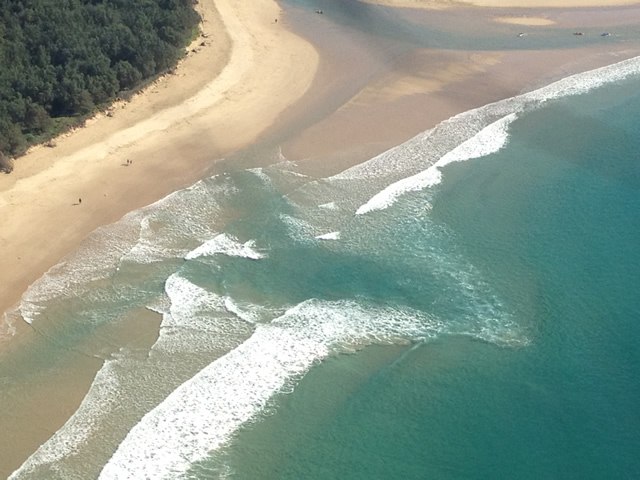
\includegraphics[width=1\linewidth]{img/Rip_C.JPG}\hfill
        \end{figure}
        \column{0.5\textwidth}
        \begin{figure}
          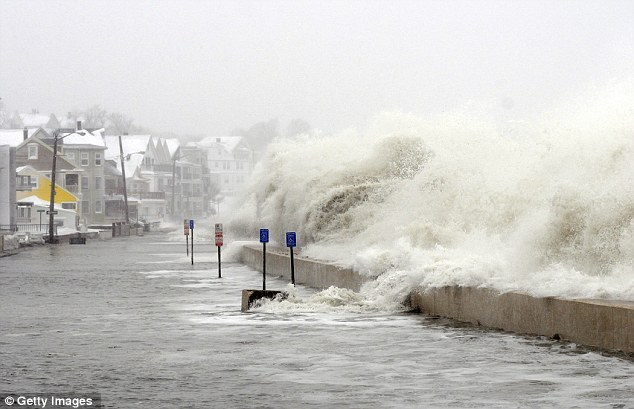
\includegraphics[width=1\linewidth]{img/C_Flood.jpg}\vfill
          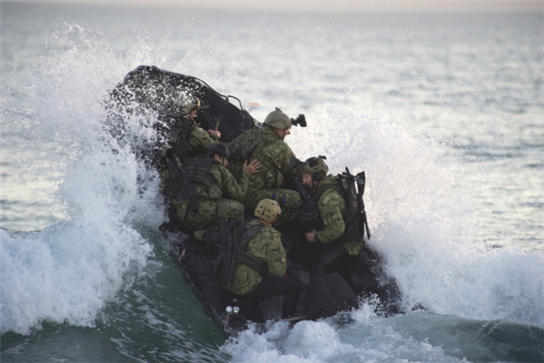
\includegraphics[width=1\linewidth]{img/Navy_S.jpg}
        \end{figure}
      \end{columns}
    \end{frame}


    %======================================================================================
    % SLIDE 3
    %======================================================================================
    \begin{frame}
      \frametitle{Bathymetry is submarine topography}
      \begin{figure}[h]
        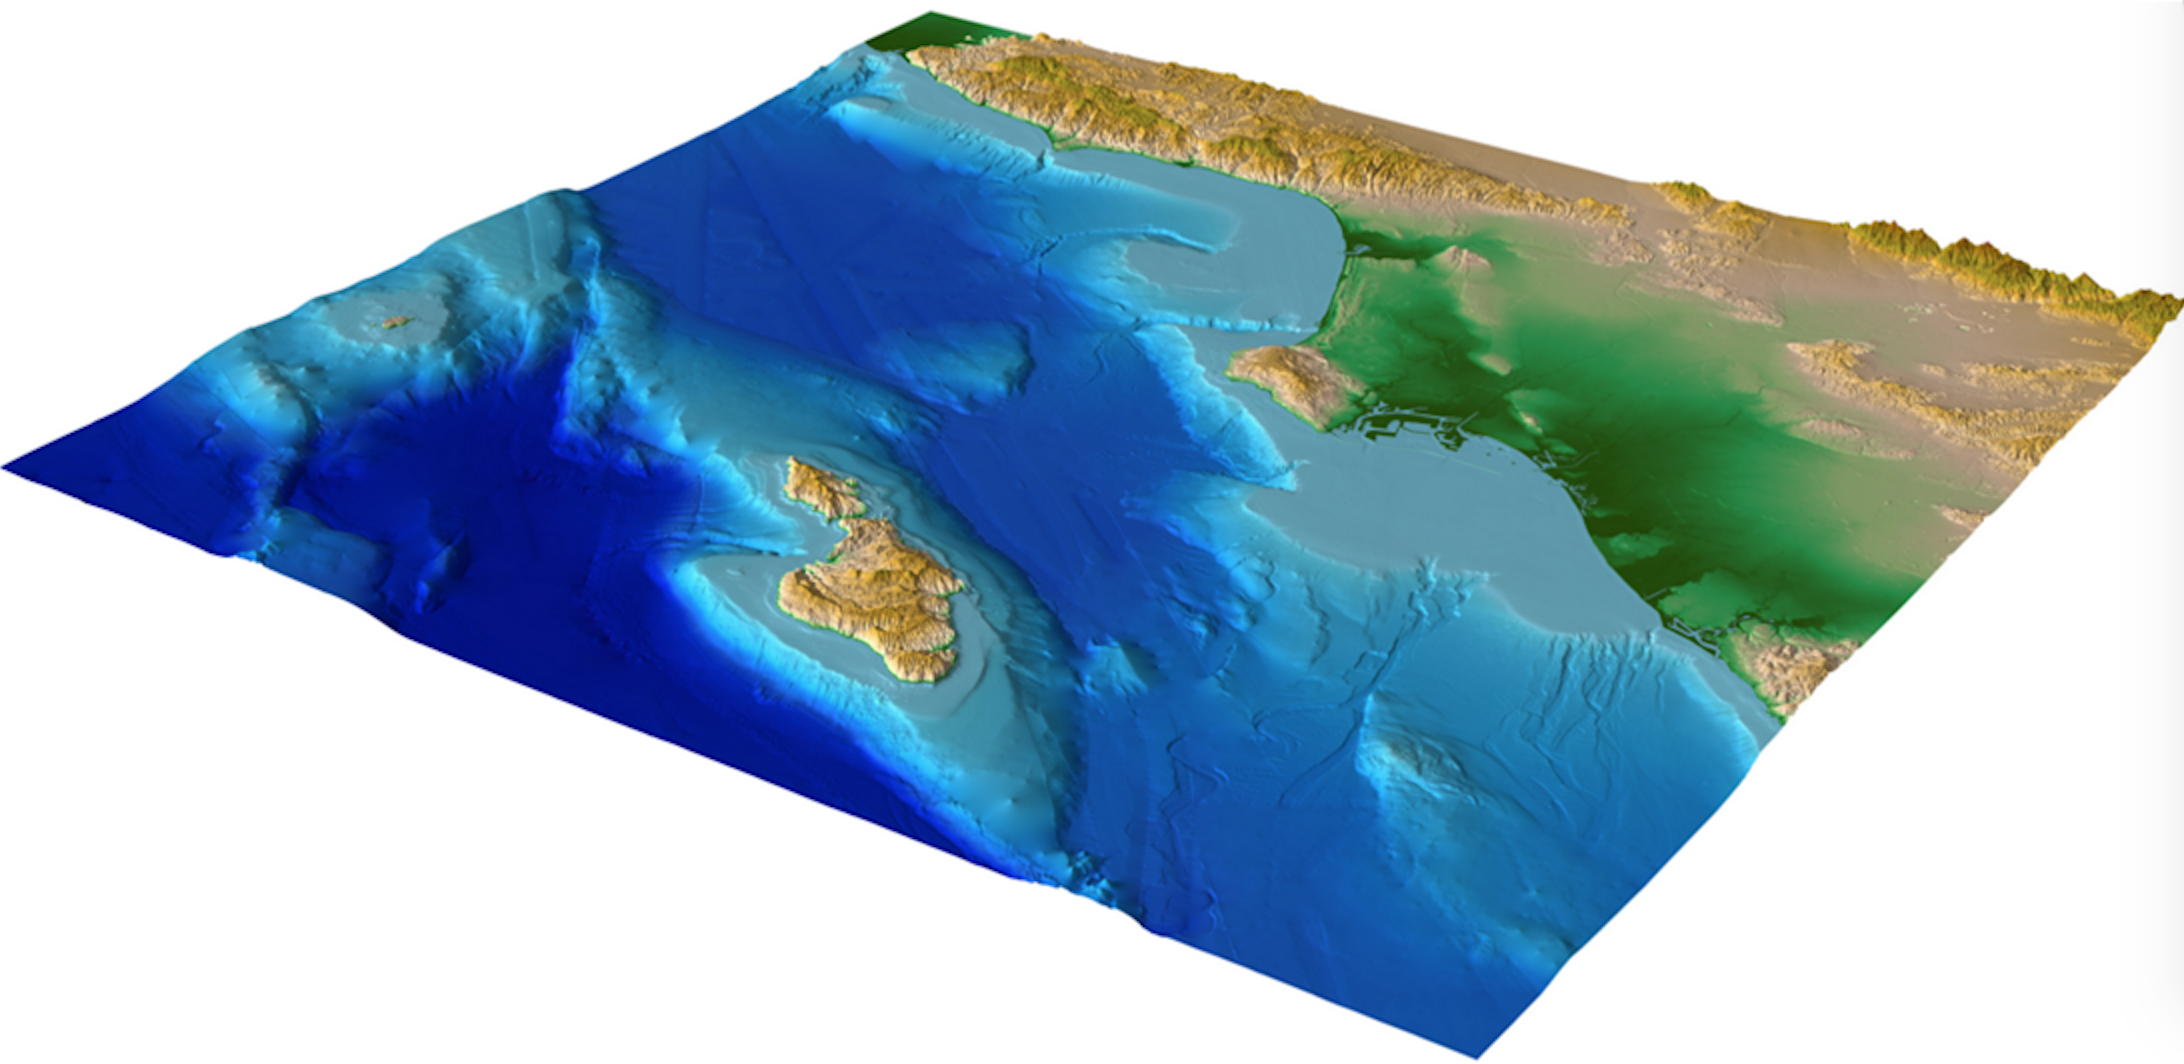
\includegraphics[width=1.\linewidth]{img/bath_topo_example.png}\hfill
      \end{figure}
    \end{frame}

    %=====================================================================================
    % SLIDE 4
    %======================================================================================
    \begin{frame}
      \frametitle{Direct measurements are expensive and challenging}
      \begin{columns}
        \column{0.5\textwidth}
        \centering
        \begin{figure}[h!]
          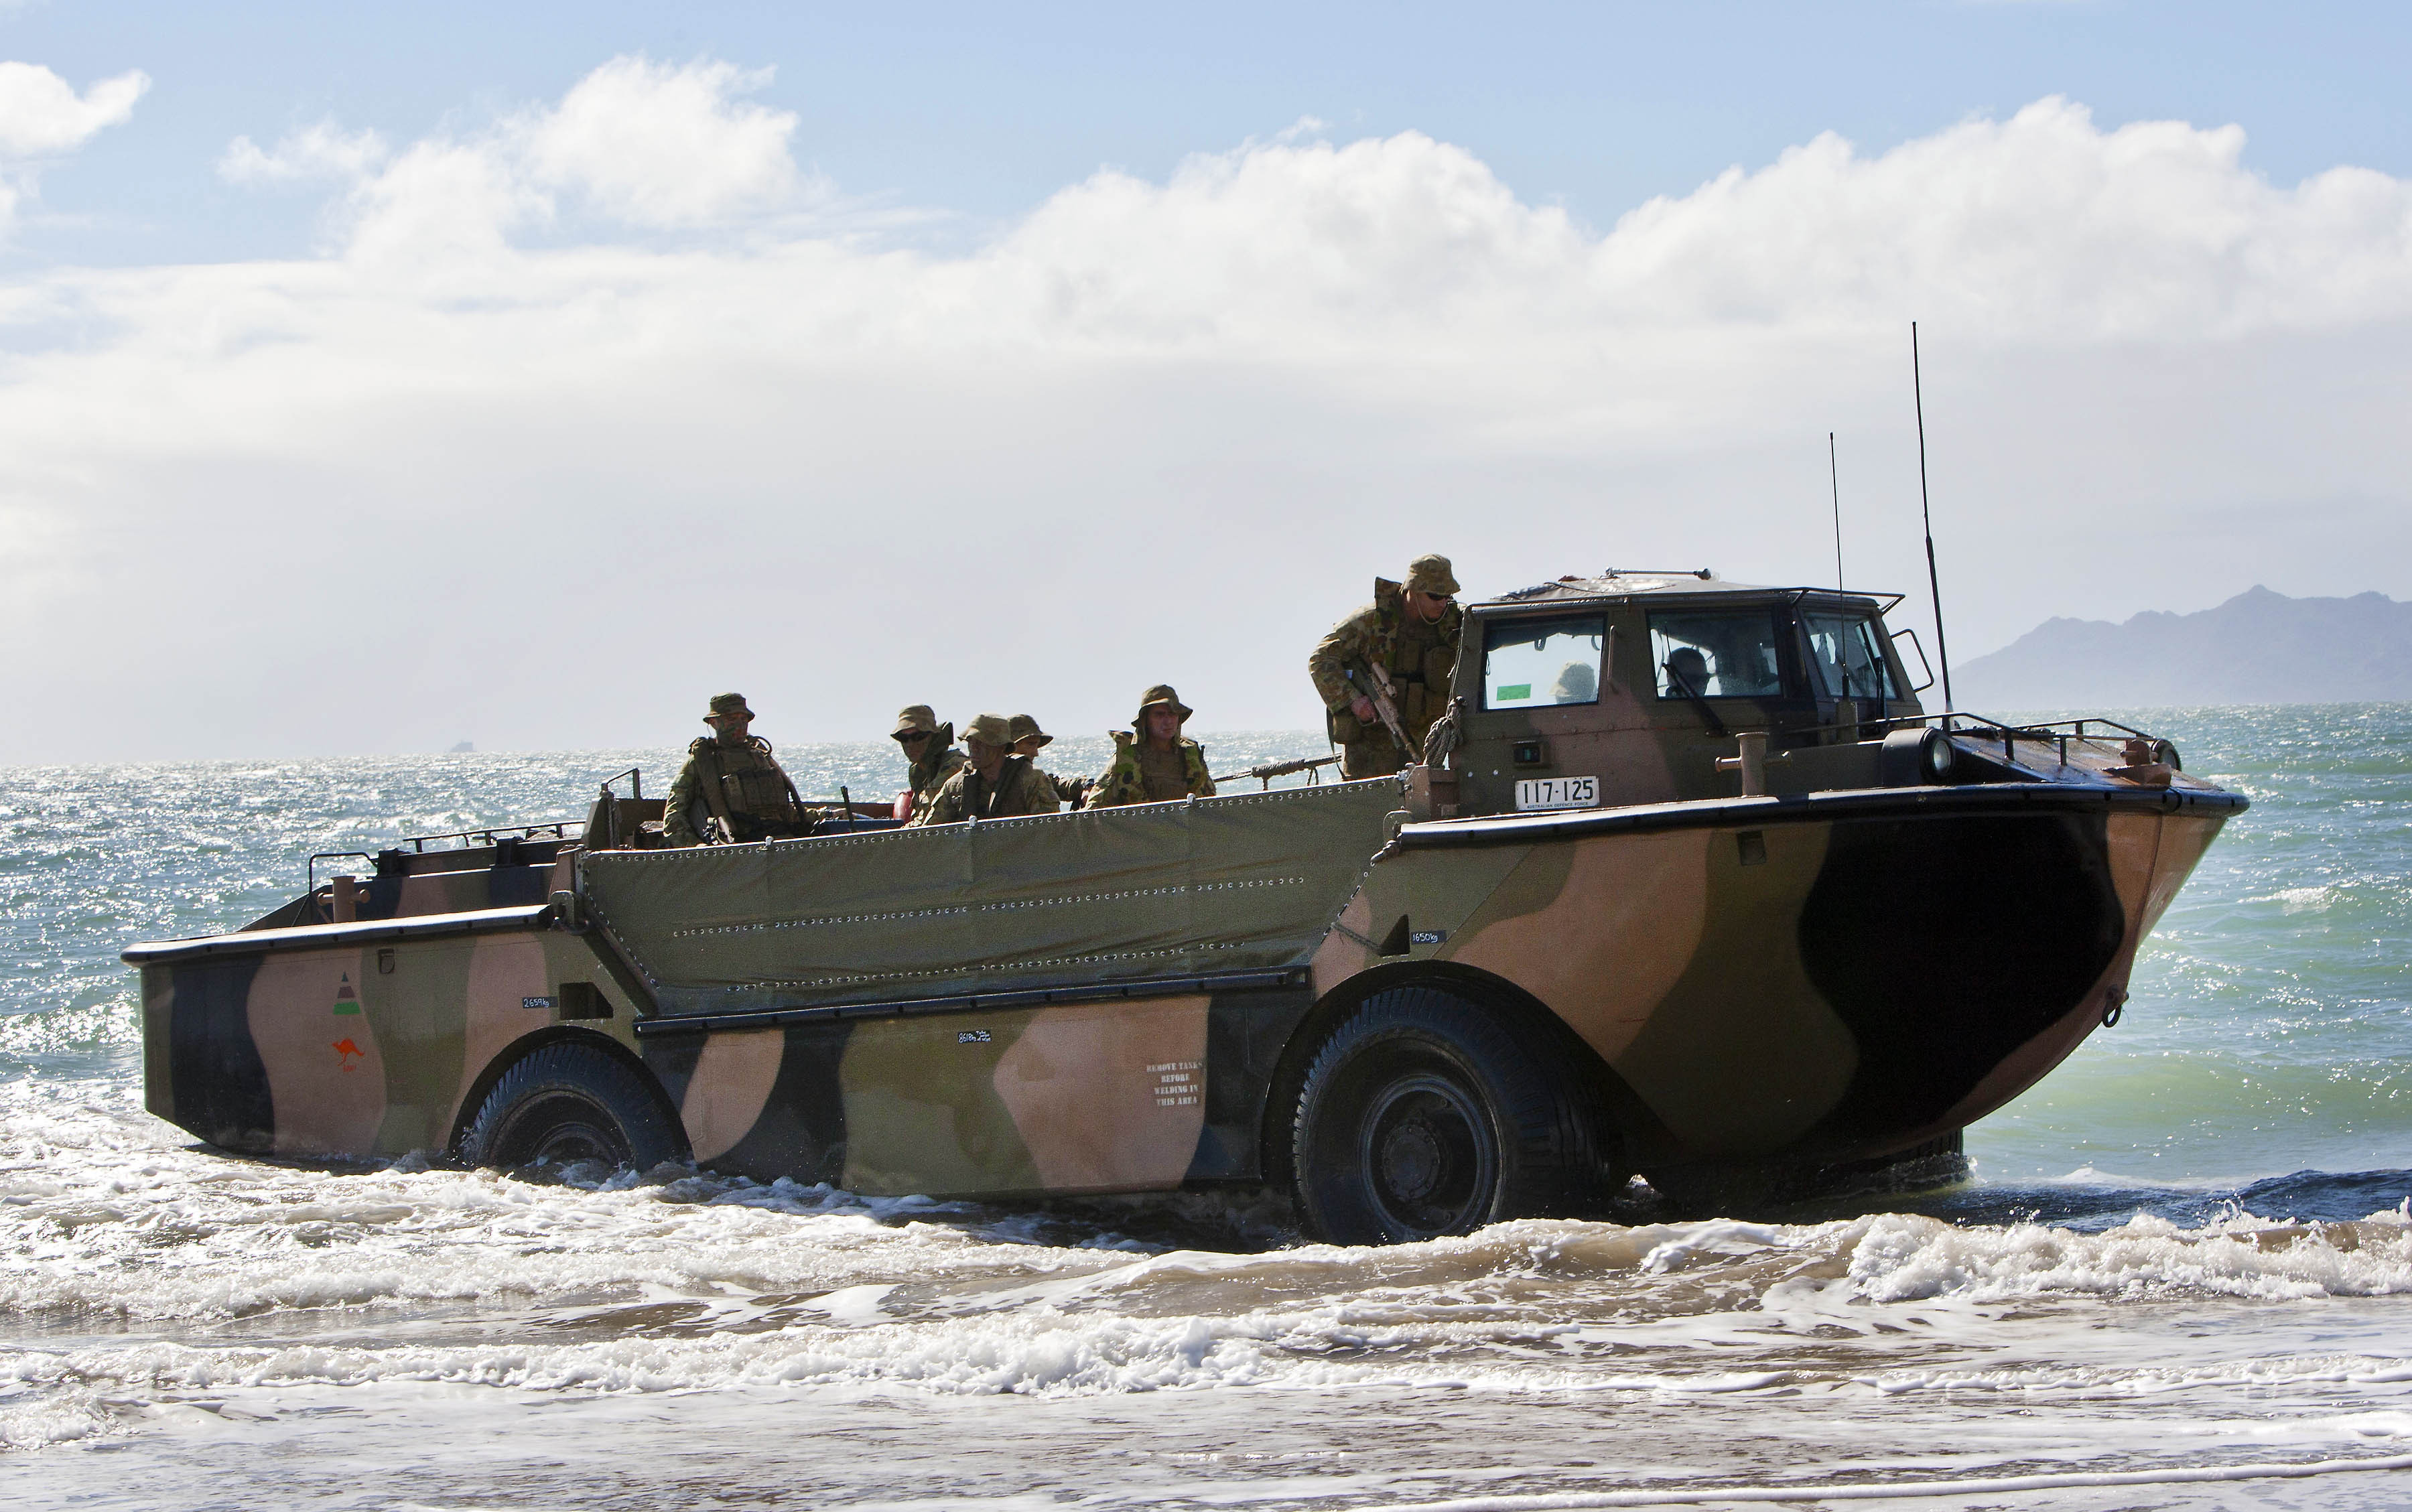
\includegraphics[width=1\linewidth]{img/LARC2.jpg}\hfill
          \centering
          \captionsetup{labelformat=empty}
          \caption{LARC}
        \end{figure}
        \column{0.5\textwidth}
        \begin{figure}[h]
          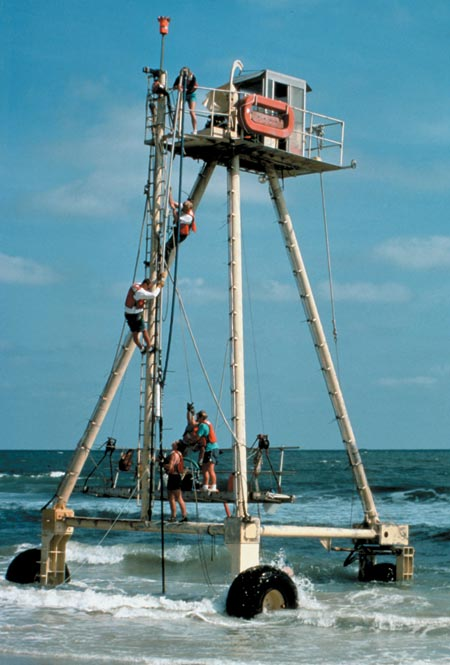
\includegraphics[width=0.8\linewidth]{img/CRAB3.jpg}
          \captionsetup{labelformat=empty}
          \caption{CRAB}
        \end{figure}
      \end{columns}
    \end{frame}

    %=====================================================================================
    % SLIDE 5
    %=====================================================================================
    \begin{frame}
      \frametitle{Inverse models estimate depth using data \& physics}

      \begin{figure}[H]
        \centering
        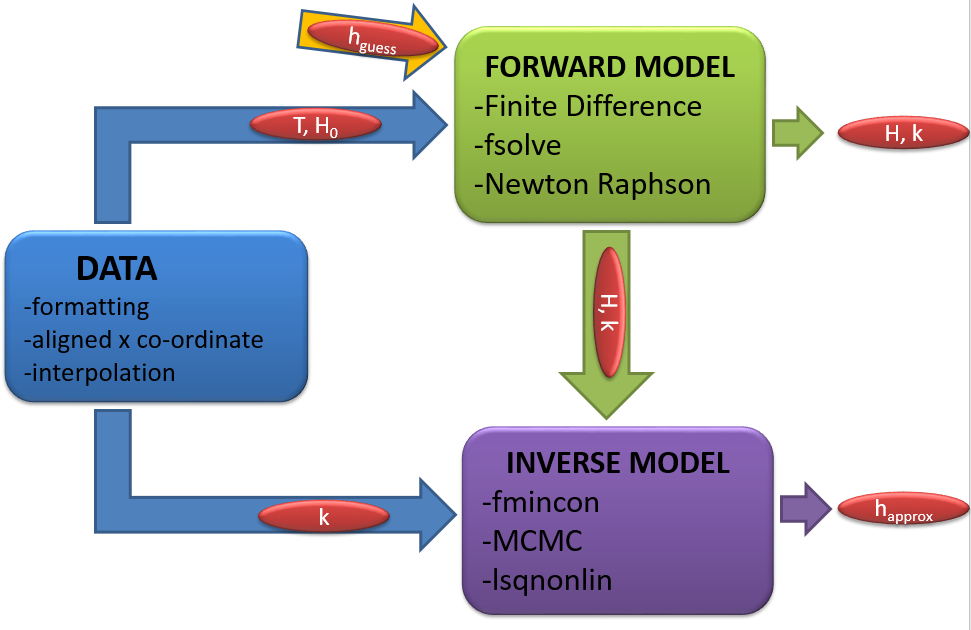
\includegraphics[width=1.0\linewidth]{img/Flow_C.png}
      \end{figure}
    \end{frame}

    %=====================================================================================
    %SLIDE  6
    %=====================================================================================
    \begin{frame}
      \frametitle{Bathymetry is related to surface wave properties}
      \begin{figure}[flowchart]
        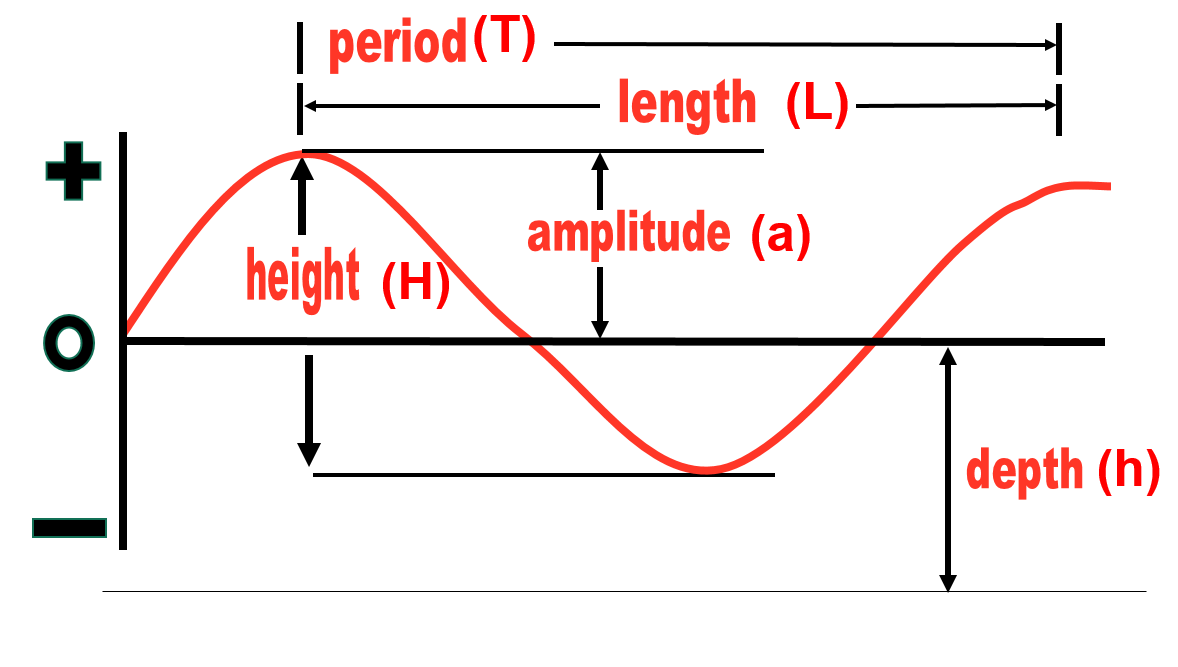
\includegraphics[width=1.0\linewidth]{img/Wave.jpg}
      \end{figure}
      \centering
      \begin{equation*}
        \textrm{wave number: } k = \frac{2\pi}{L}
      \end{equation*}
    \end{frame}

    %====================================================================================
    %====================================================================================
    \section{Data}
    %====================================================================================
    %====================================================================================

    %====================================================================================
    % SLIDE  7
    %====================================================================================
    \begin{frame}
      \frametitle{Before we invert we need data}
      \begin{figure}[flowchart]
        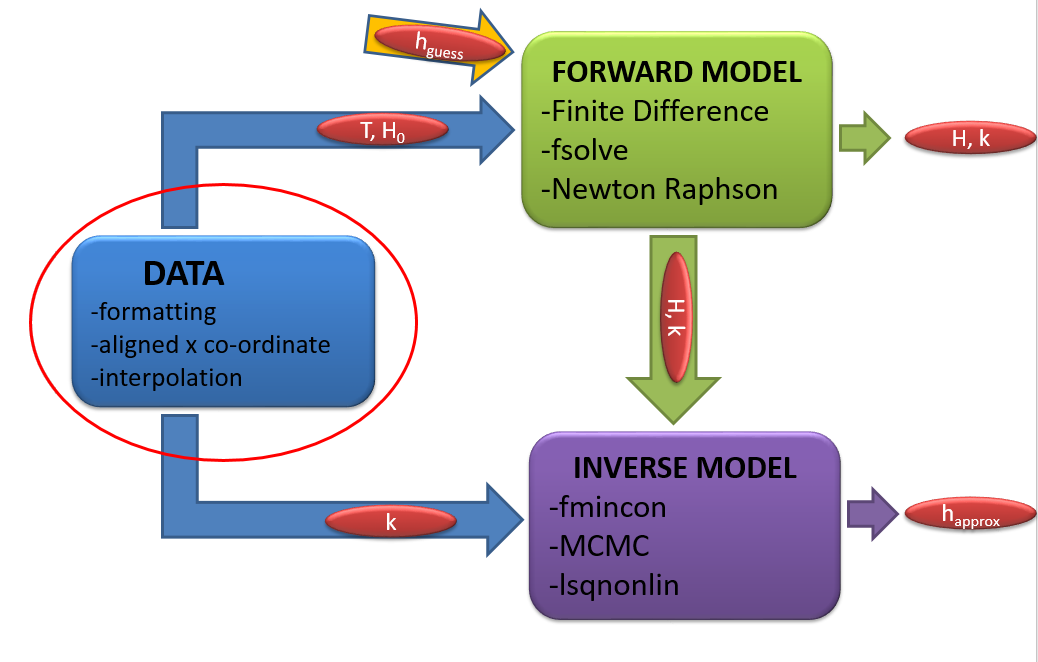
\includegraphics[width=1.0\linewidth]{img/Focus_D.png}
      \end{figure}
    \end{frame}

    %====================================================================================
    %SLIDE   8
    %====================================================================================
    \begin{frame}
      \frametitle{Data was collected by the  USACE in Duck, NC}
      \centering
      \begin{figure}
        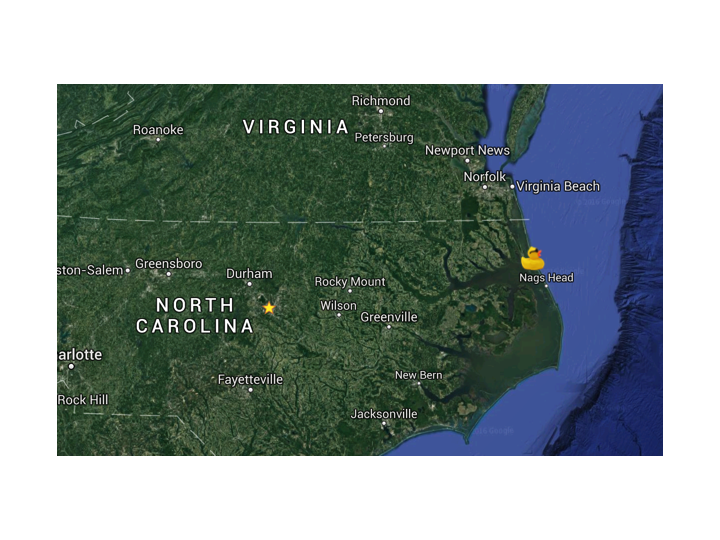
\includegraphics[width=1\linewidth]{img/map_ncsu_duck.png}
      \end{figure}
    \end{frame}

    %====================================================================================
    % SLIDE 9
    %====================================================================================
    \begin{frame}
      \frametitle{Model coordinate system has $x = 0~m$ offshore}
      \begin{figure}[H]
        \centering
        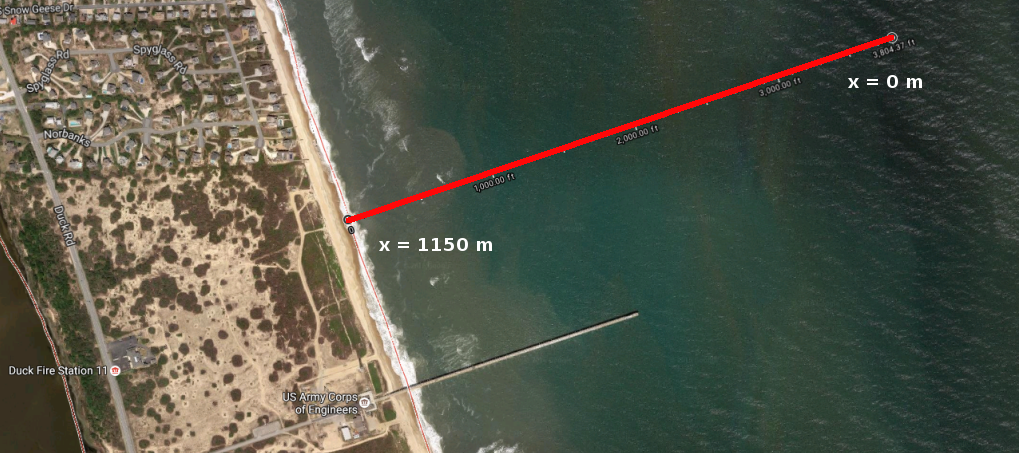
\includegraphics[width=1\linewidth]{img/Transect.png}
      \end{figure}
    \end{frame}


    %====================================================================================
    % SLIDE 10
    %====================================================================================
    \begin{frame}
      \frametitle{Remote sensing of surface properties are possible}
      \begin{columns}
        \column{0.5\textwidth}
        \begin{figure}[H]
          \centering
          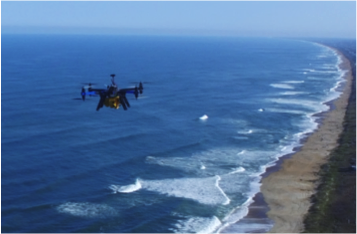
\includegraphics[width=1\linewidth]{img/remoteSensingUAV.png}
        \end{figure}
        \column{0.5\textwidth}
        \begin{figure}[H]
          \centering
          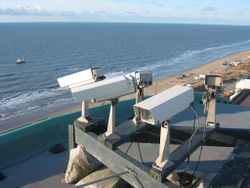
\includegraphics[width=0.9\linewidth]{img/argus_camera.JPG}
        \end{figure}
      \end{columns}
    \end{frame}

%====================================================================================
% SLIDE 11
%====================================================================================
\begin{frame}
	\frametitle{Data includes $T$, $H$ at offshore boundary; 1D $k$}
		\begin{figure}[H]
			\centering
			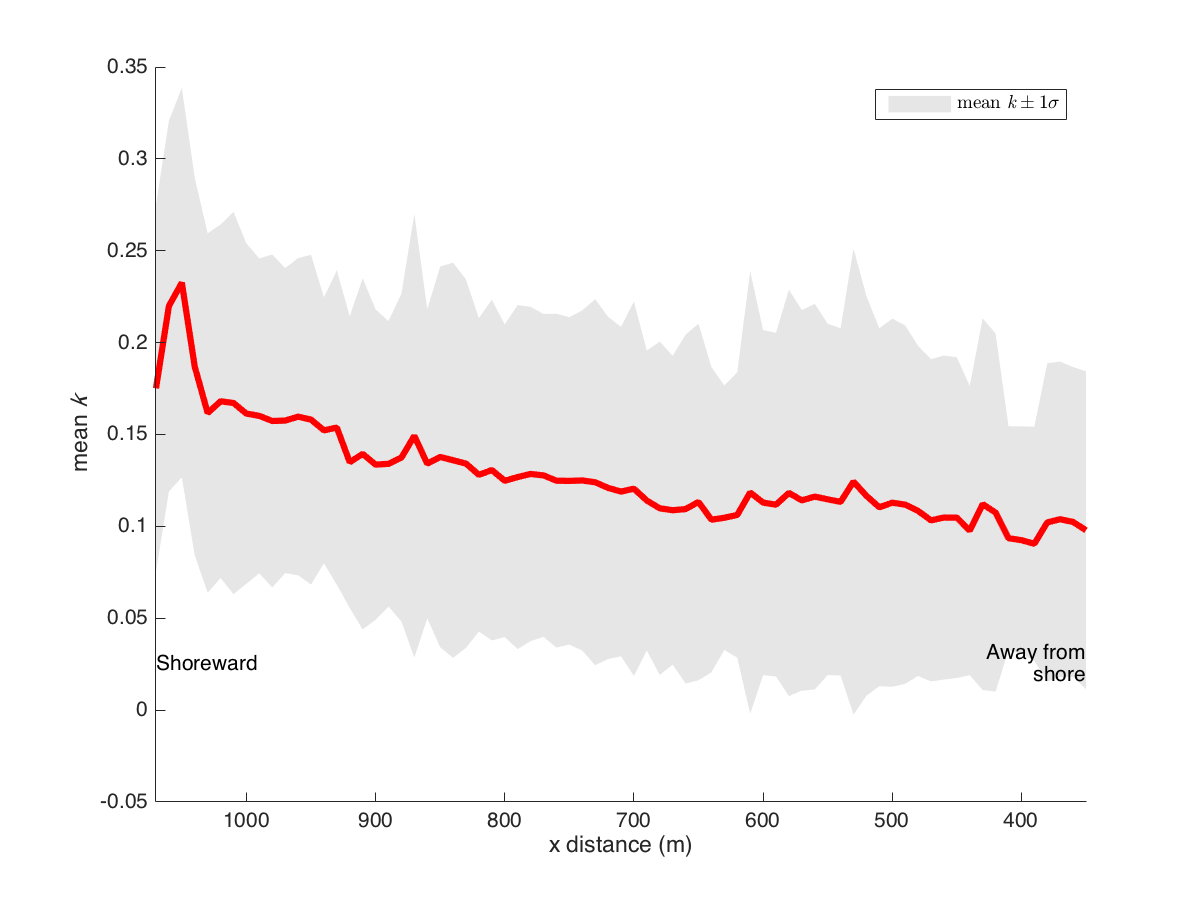
\includegraphics[width=1\linewidth]{img/k1Dmean_std.png}
		\end{figure}
\end{frame}

%====================================================================================
% SLIDE 12
%====================================================================================
\begin{frame}
	\frametitle{Known bathymetry is used for testing our results}
%		\begin{columns}
%			\column{0.5\textwidth}
			\begin{figure}[H]
	 			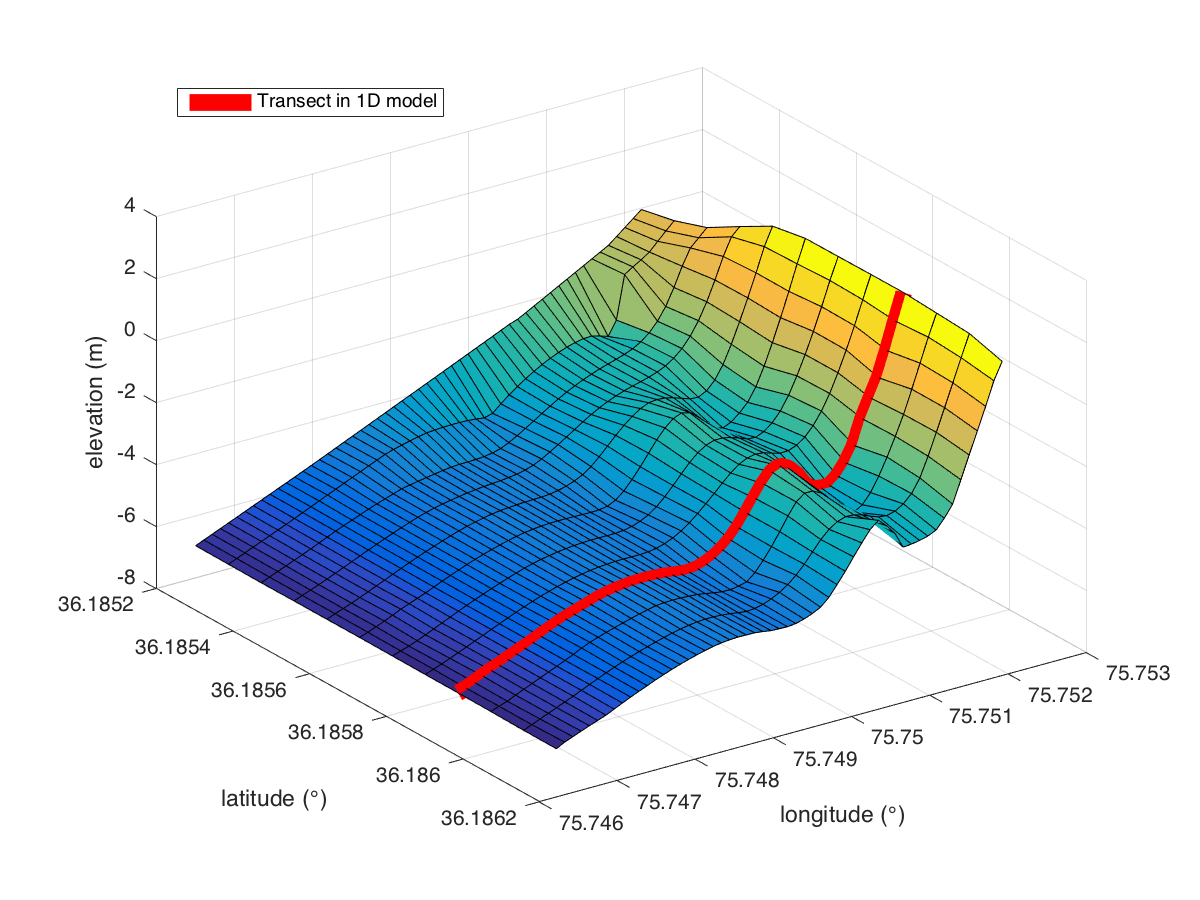
\includegraphics[width=1\linewidth]{img/trueBath2D.png}
	 		\end{figure}
%			\column{0.5\textwidth}
%				\begin{figure}[h]
%					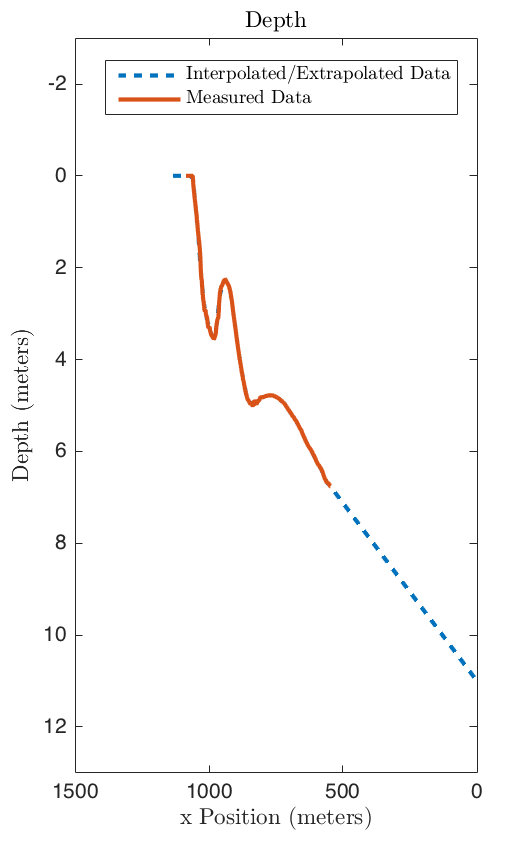
\includegraphics[width=.70\linewidth]{img/DepthChart.png}
%				\end{figure}
%			\end{columns}
\end{frame}

%==================================================================================
%==================================================================================
\section{Forward Model}
%==================================================================================
%==================================================================================

%==================================================================================
% SLIDE 13
%==================================================================================
\begin{frame}
 	\frametitle{Forward model computes $k$ assuming $h_{guess}$ \& BC}
		\begin{figure}[H]
	 		\centering
	 		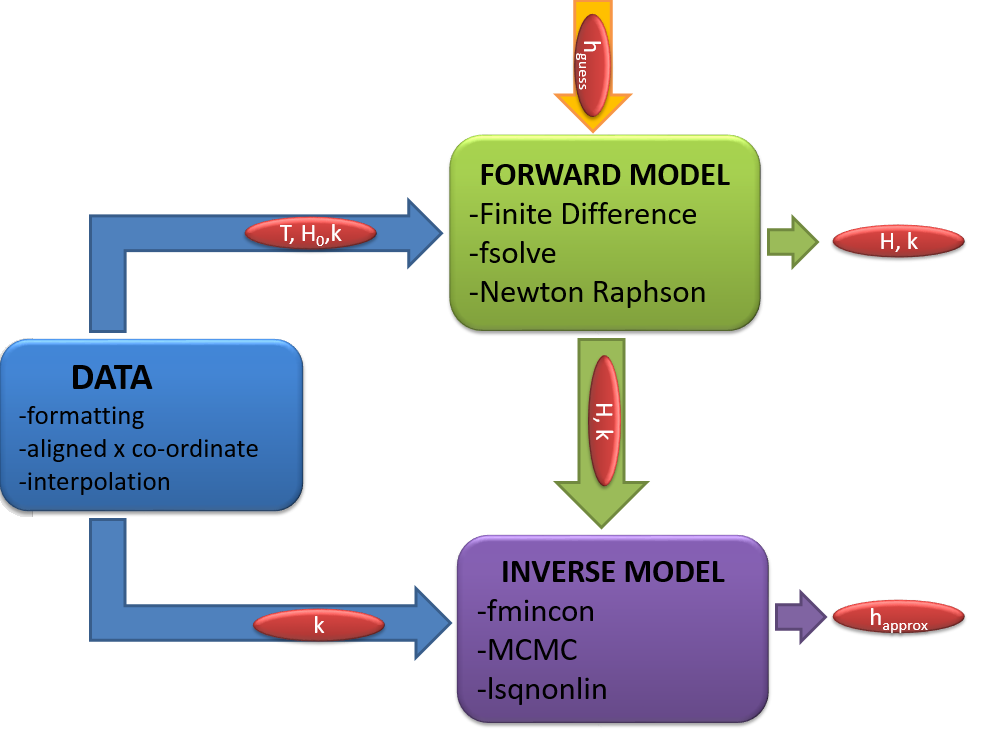
\includegraphics[width=1.0\linewidth]{img/Flow_New.png}
	 	\end{figure}
\end{frame}

%==================================================================================
% SLIDE 14
%==================================================================================
\begin{frame}
	\frametitle{Wave dispersion relationship relates $k$ to $h$}
		Dispersion Relation [1]:
		$$ \sigma^2=gk\tanh(kh) \Longleftrightarrow \left(\frac{2\pi}{T}\right)^2 = g\left(\frac{2\pi}{L}\right) tanh \left(\frac{2\pi h}{L}\right)
		$$
		\begin{itemize}
			\item Relates wave number $(k)$ and Period $(T)$
			\item Wave length $(L)$ varies with depth $(h)$
			\item Period $(T)$ remains constant
		\end{itemize}
\end{frame}


%==================================================================================
% SLIDE 15
%==================================================================================
\begin{frame}
	\frametitle{1D forward model relates $H$ and $h$}
	Energy Flux Method [2]:
	$$\frac{d}{dx}\left(EC_g\right)=-\delta $$
	\begin{itemize}
	    \item Relates wave height $(H)$ and wave number $(k)$
		\item $E(\rho,g,{\bf H})$: Wave Energy
		\item  $C_{g}(\rho,{\bf k},h)$: Group celerity
		\item $\delta(\rho,g,T,{\bf H}):$ $^3$Wave energy dissipation function
	\end{itemize}
	$\quad$\\
	\begin{flushright}
	{\tiny $^1$Dean et al, 2000 (pg 64), $^2$Edward et al, 1983 (pg 2) and $^3$Alex et al, 2008 (pg 2)}.
	\end{flushright}
\end{frame}
%==================================================================================
%  SLIDE 16
%==================================================================================
\begin{frame}
	\frametitle{1D forward model Results}
	   \begin{columns}[t]
        \column{.5\textwidth}
        \centering
        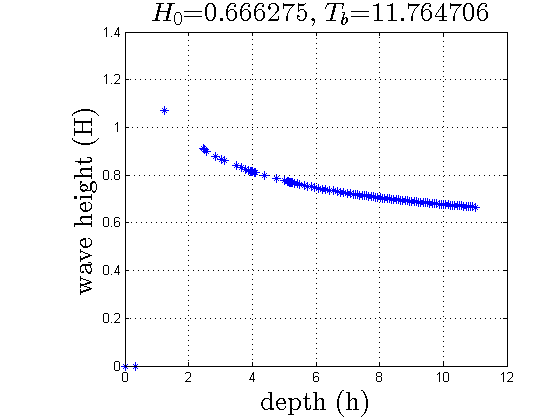
\includegraphics[width=5.5cm,height=3.5cm]{img/Wave_height_Depth.png}\\
        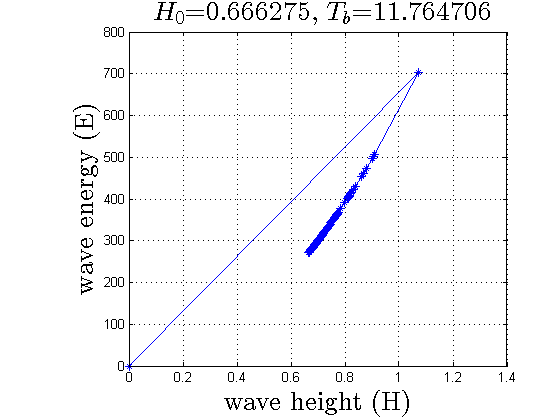
\includegraphics[width=5.5cm,height=3.5cm]{img/Wave_energy_WaveHeight.png}
        \column{.5\textwidth}
        \centering
       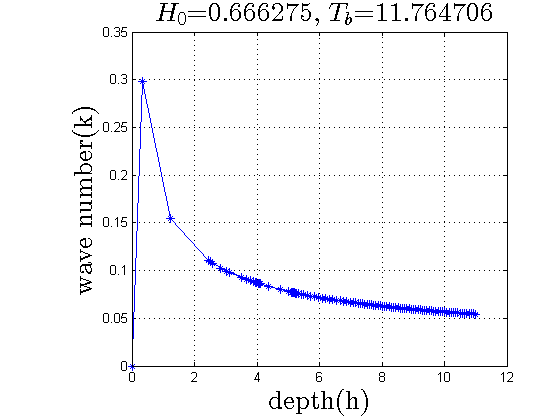
\includegraphics[width=5.5cm,height=3.5cm]{img/Wave_number_Depth.png}\\
       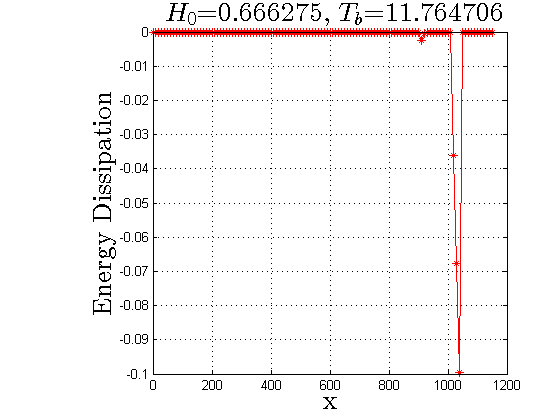
\includegraphics[width=5.5cm,height=3.5cm]{img/Energy_Dissipation_x.png}
      \end{columns}
\end{frame}

%==================================================================================
%==================================================================================
\section{Inverse Methods}
%==================================================================================
%==================================================================================

%==================================================================================
% SLIDE 16
%==================================================================================
\begin{frame}
 	\frametitle{Invert for bathymetry given surface data \& physics}
		\begin{figure}
			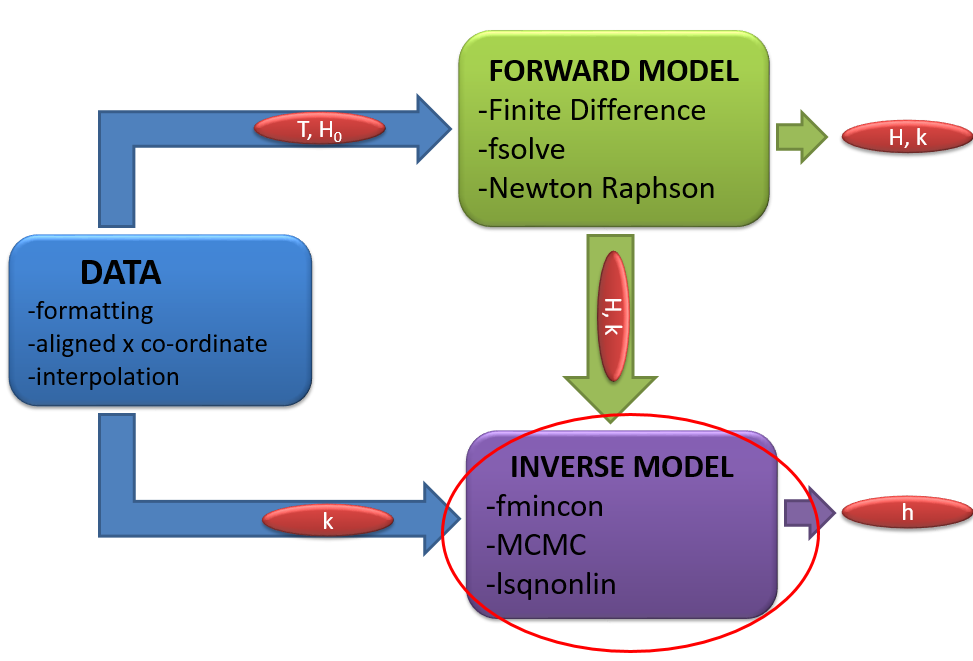
\includegraphics[width=1.0\linewidth]{img/INV.png}
		\end{figure}
\end{frame}

%==================================================================================
% SLIDE 17
%==================================================================================
\begin{frame}
	\frametitle{Solutions are computed using 3 inversion methods}
		\centering
		\begin{enumerate}
			\item Nonlinear Least Squares (lsqnonlin)
			\begin{itemize}
				\item Logical place to start
			\end{itemize}
			$\,$\\
			\item Bayesian MCMC (Metropolis)
			\begin{itemize}
				\item Gives a distribution of depth estimates
			\end{itemize}
			$\,$\\
			\item Tikhonov Regularization (fmincon)
			\begin{itemize}
				\item Bounded-constraint multivariate problem
			\end{itemize}
		\end{enumerate}
\end{frame}

%==================================================================================
\subsection{Manufactured}
%==================================================================================

%==================================================================================
%  SLIDE 18
%==================================================================================
\begin{frame}
 	\frametitle{Manufactured ``data" is used to test our algorithms}
		\begin{figure}
			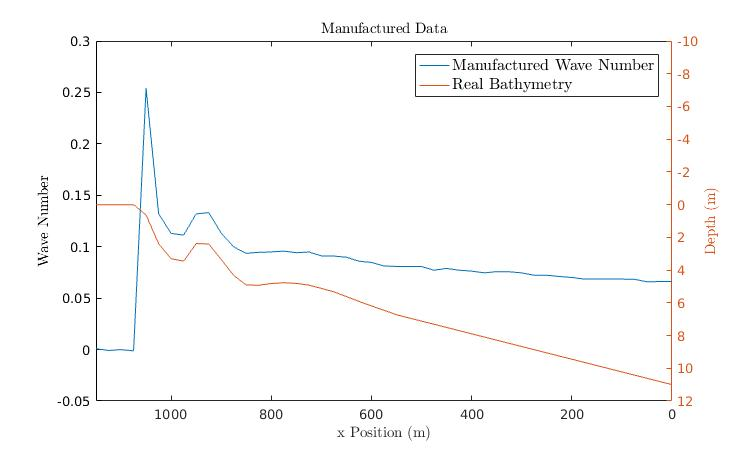
\includegraphics[width=1.0\linewidth]{img/Manufactured_data.jpg}
		\end{figure}
\end{frame}


%==================================================================================
%  SLIDE 19
%==================================================================================
\begin{frame}
	\frametitle{All methods capture the sandbar well}
	   \begin{columns}[t]
        \column{.5\textwidth}
        \centering
        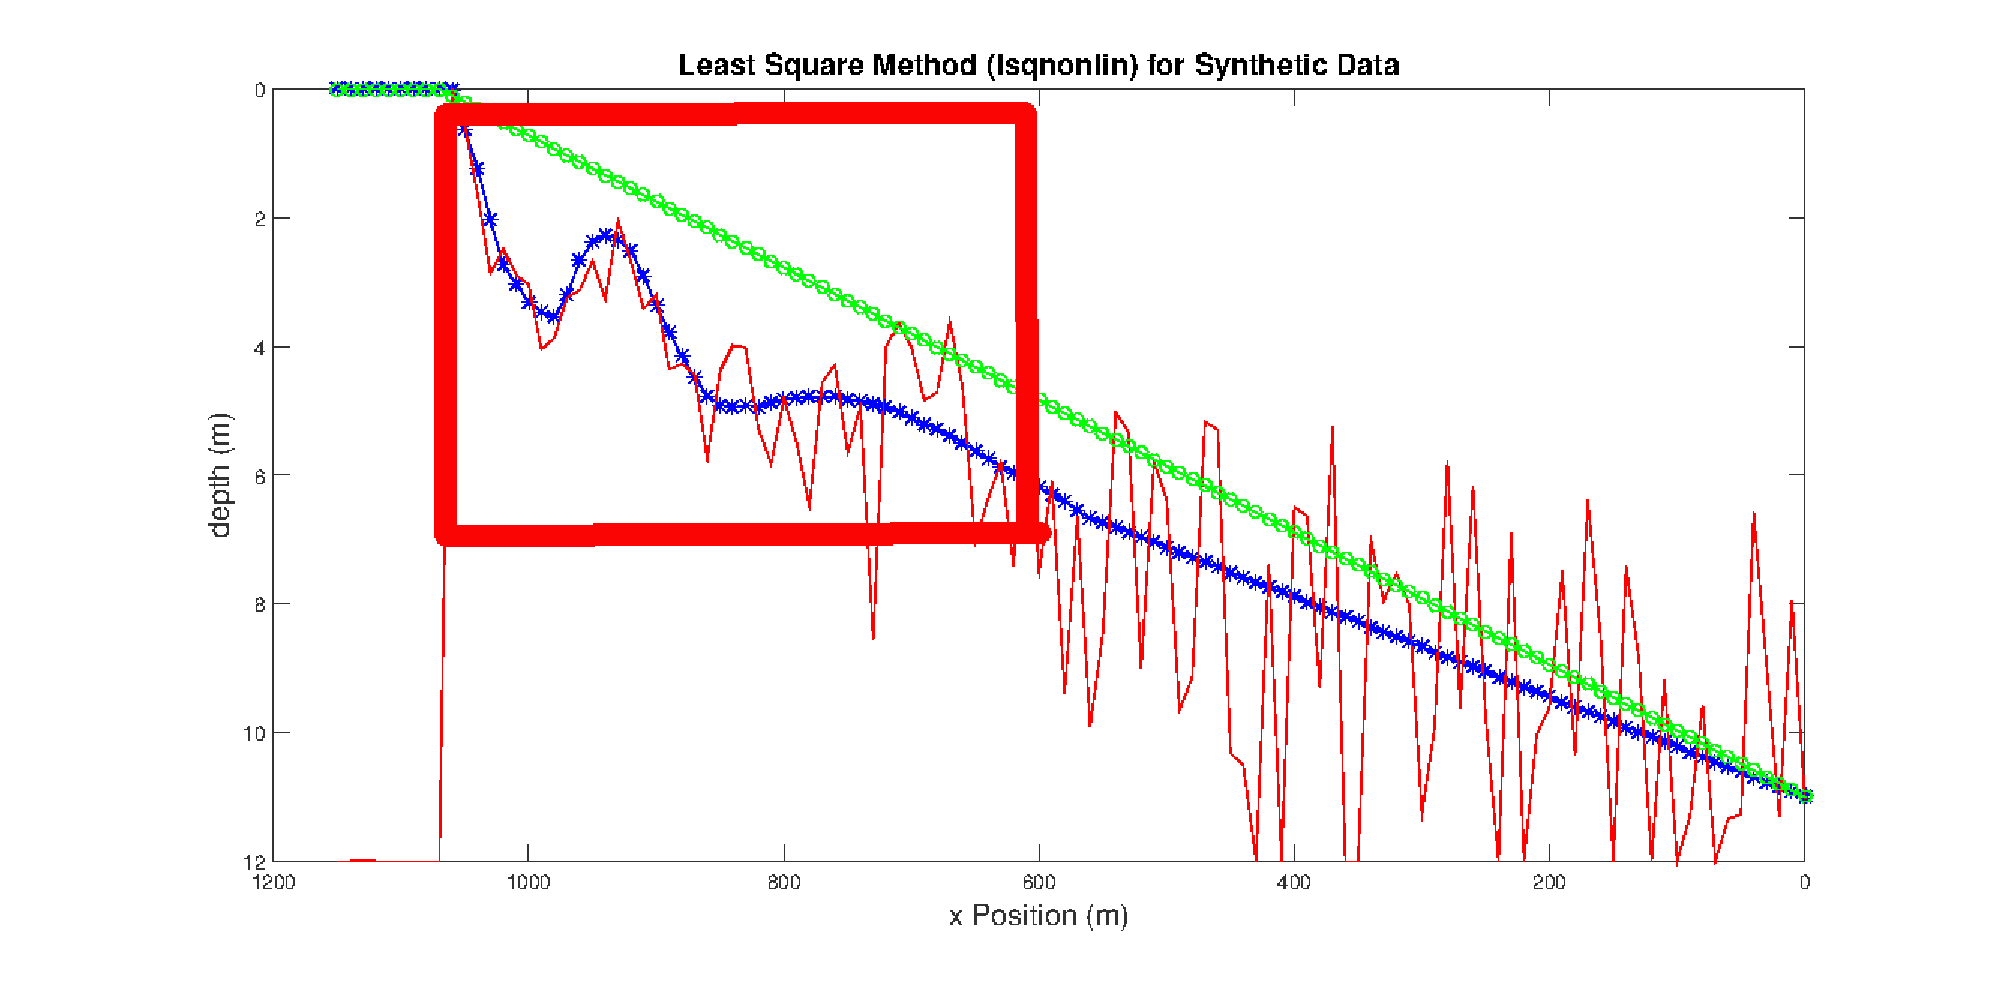
\includegraphics[width=5.5cm,height=3.5cm]{img/lsqnonlin_simulated_10m_new_box.eps}\\
        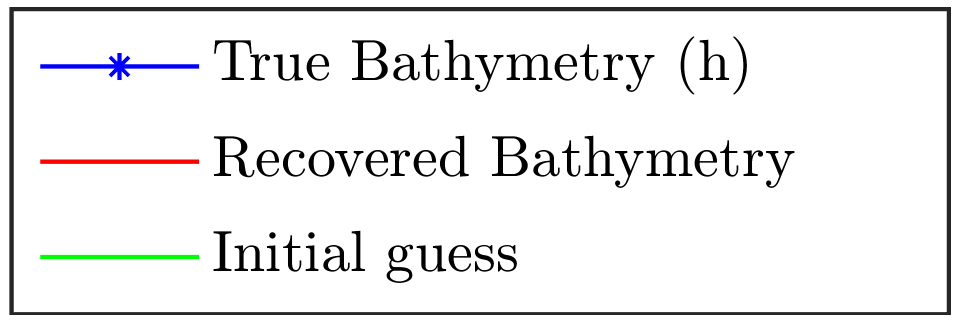
\includegraphics[width=4.0cm,height=1.5cm]{img/legend_simulated.png}
        \column{.5\textwidth}
        \centering
       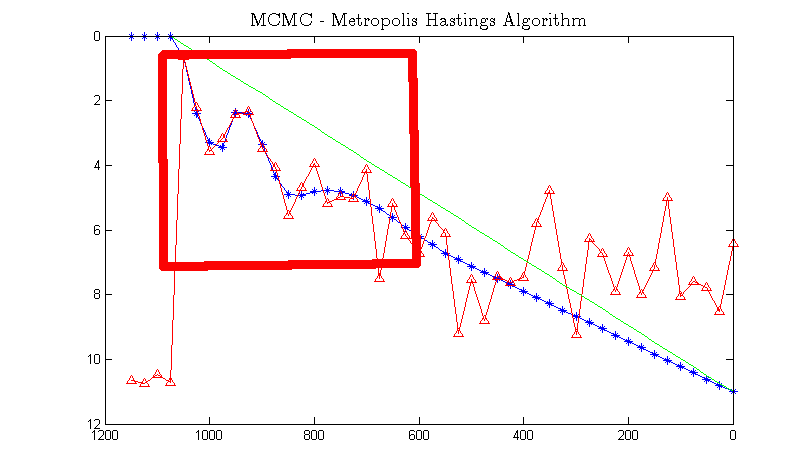
\includegraphics[width=5.5cm,height=3.5cm]{img/MCMC-manufactured_new_box.png}\\
       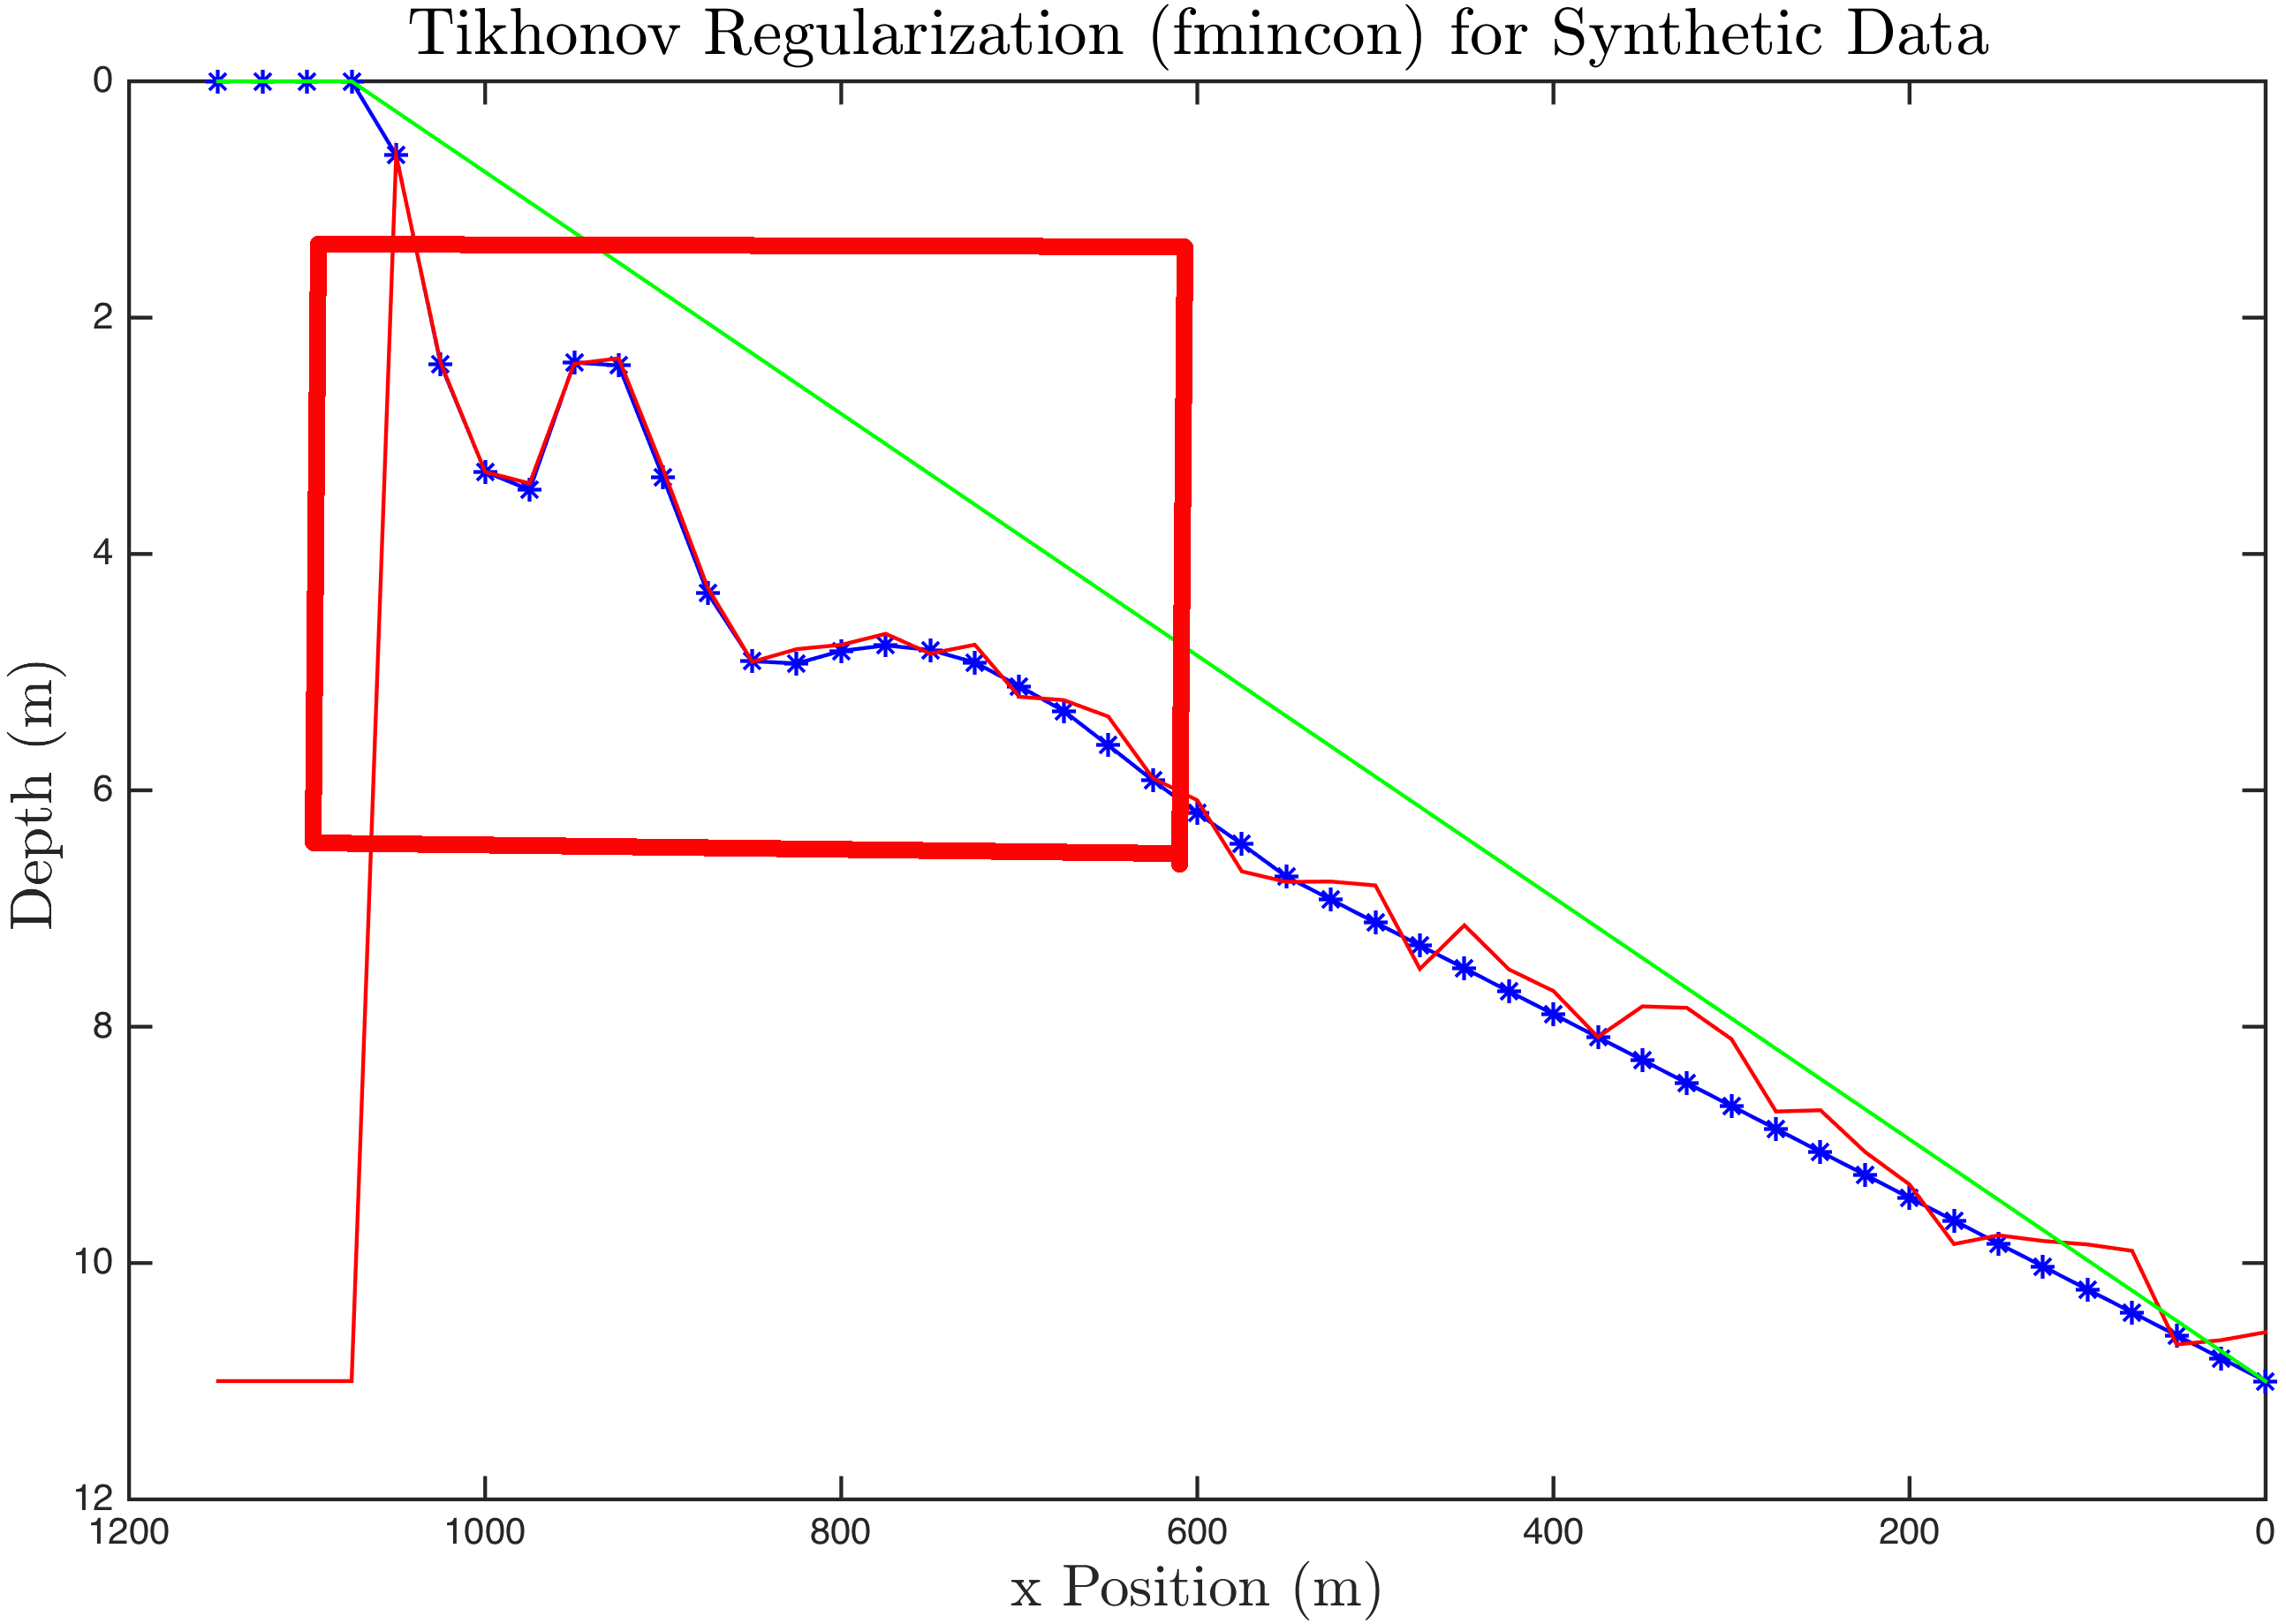
\includegraphics[width=4.8cm,height=3.5cm]{img/fmincon_simulated_25m_new_box.png}
      \end{columns}
\end{frame}

%==================================================================================
\subsection{Real}
%==================================================================================

%===================================================================================
% SLIDE 20
%===================================================================================
\begin{frame}
	\frametitle{Real $k$ data is selected for a period with low noise}
		\begin{figure}
			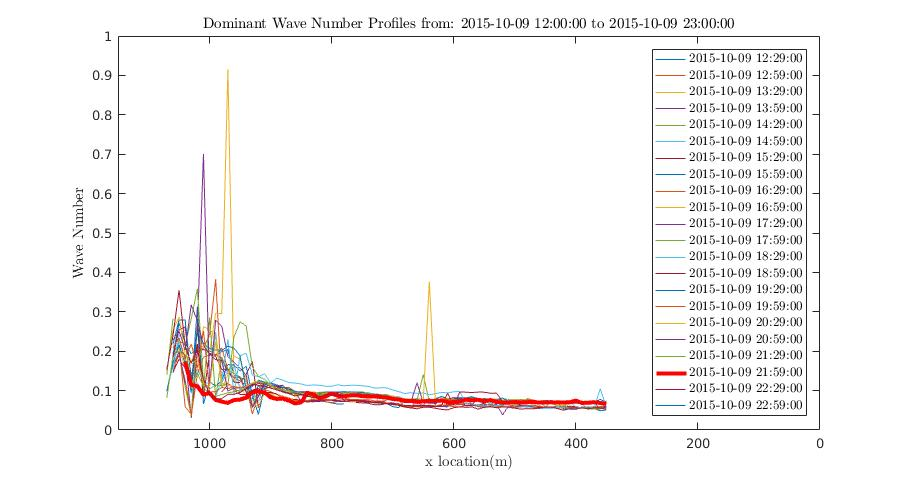
\includegraphics[width=1.0\linewidth]{img/Real_k_data.jpg}
		\end{figure}
\end{frame}


%==================================================================================
%  SLIDE 21
%==================================================================================
\begin{frame}
	\frametitle{Bathymetry estimates perform well in shallow water}
	   \begin{columns}[t]
        \column{.5\textwidth}
        \centering
        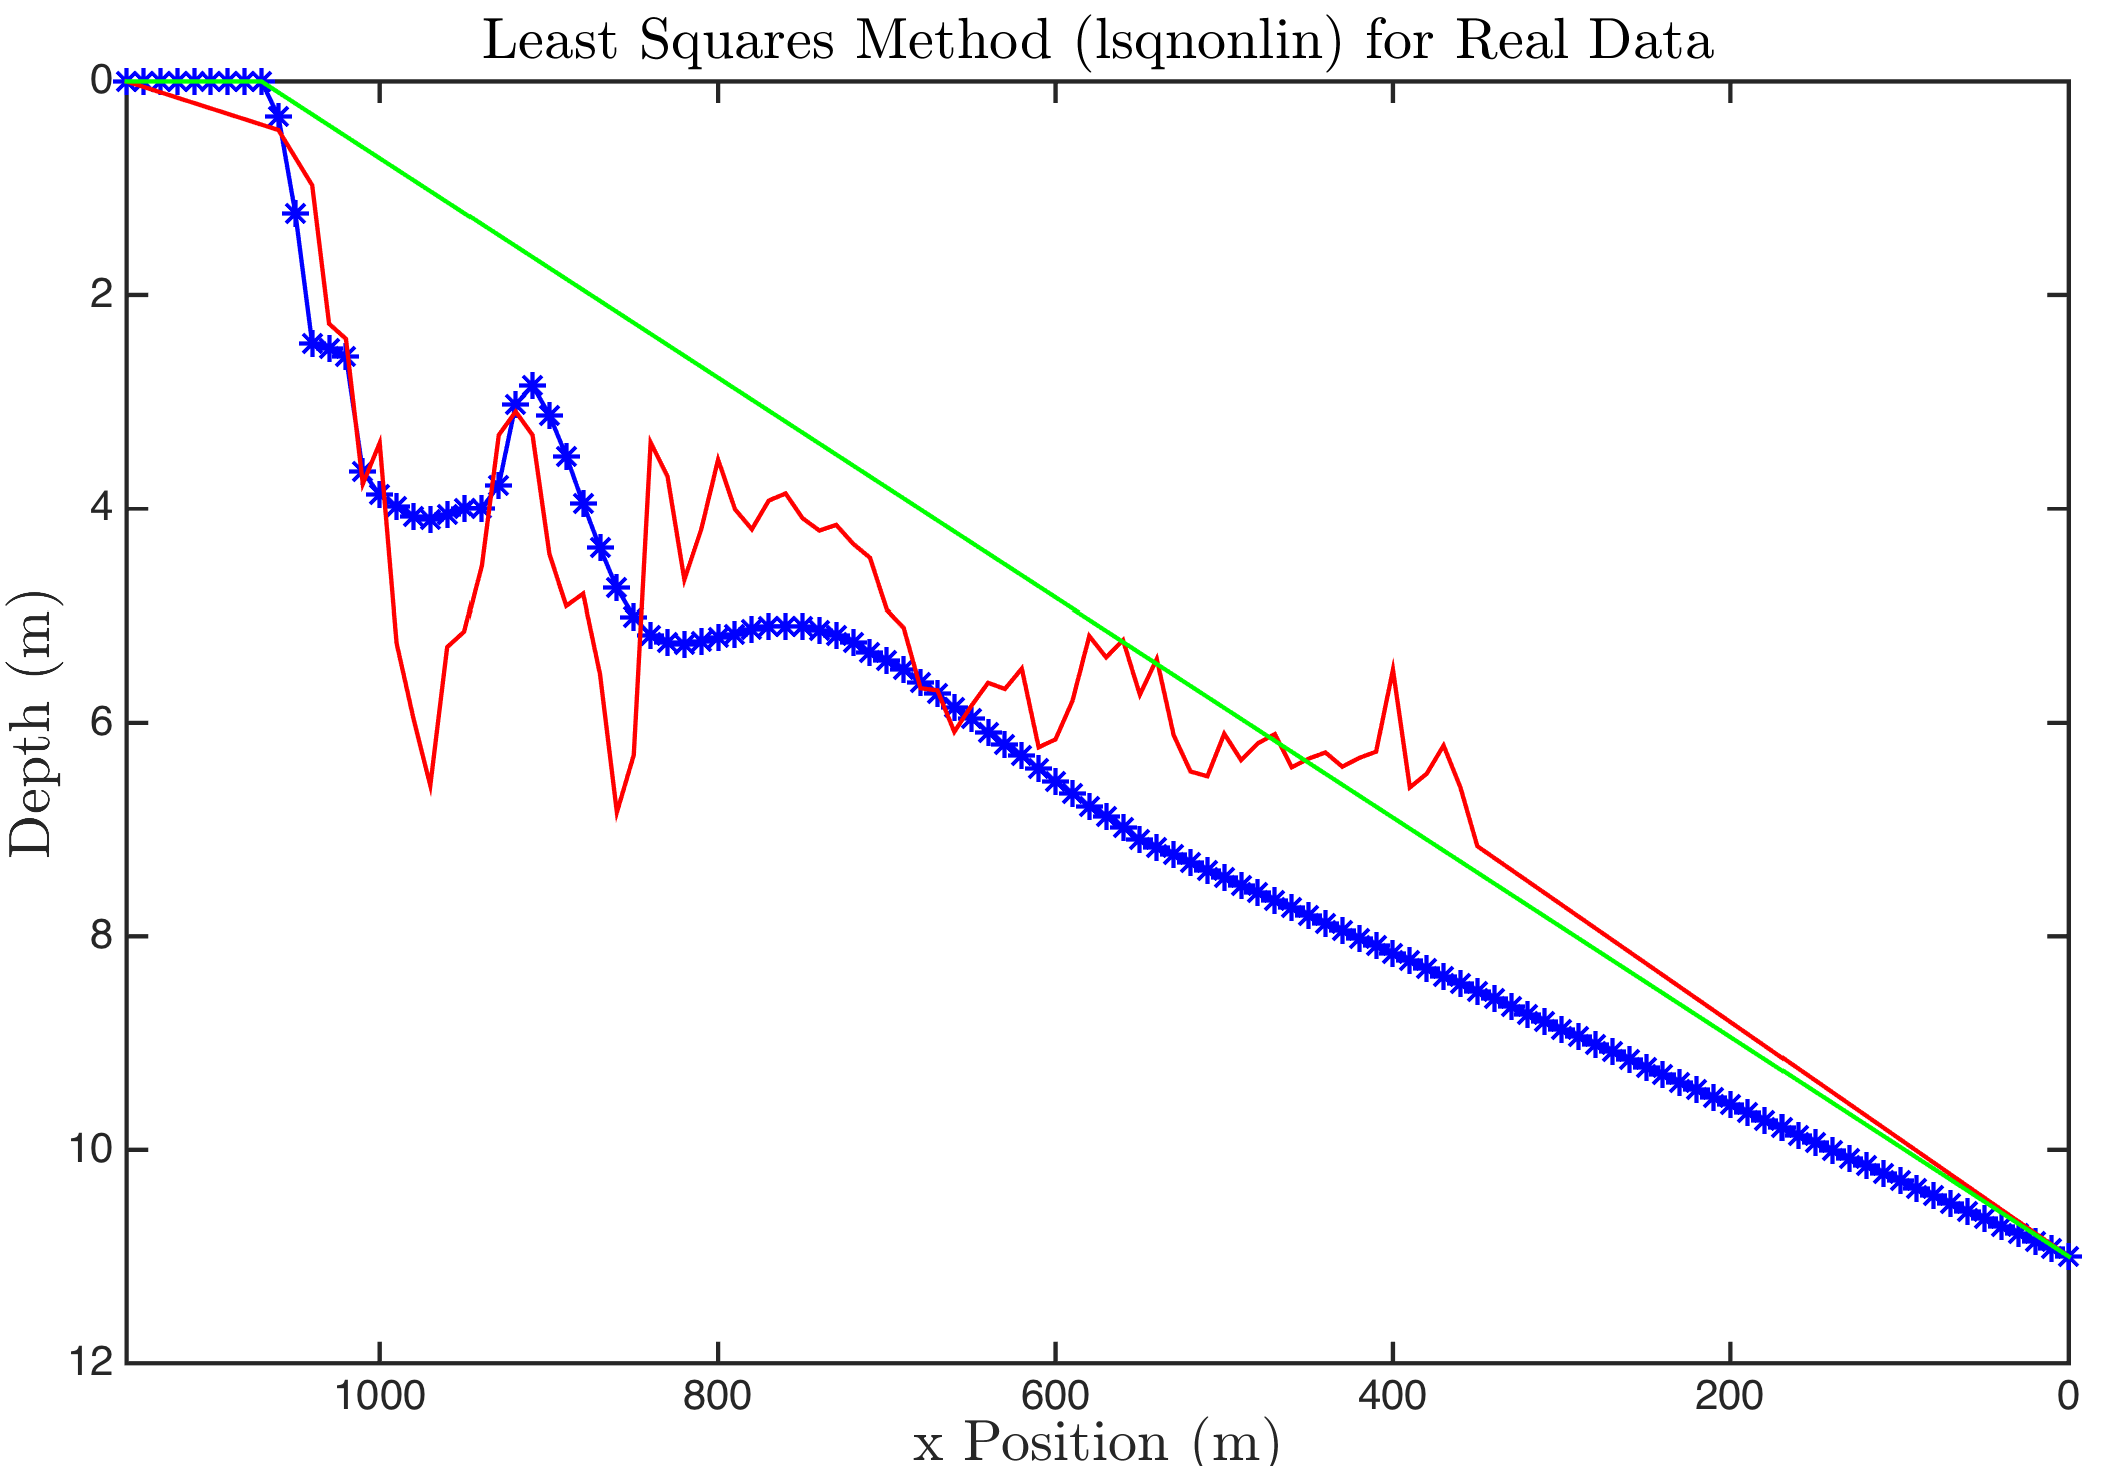
\includegraphics[width=5.2cm,height=3.5cm]{img/lsqnonlin_real_data_oct09}\\
        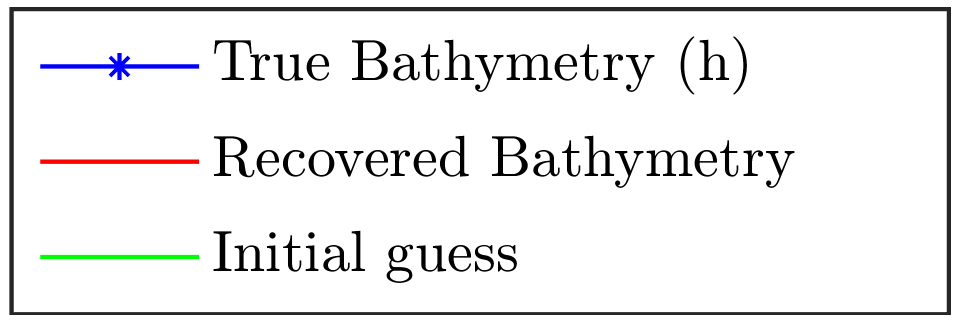
\includegraphics[width=4.0cm,height=1.5cm]{img/legend_simulated.png}
        \column{.5\textwidth}
        \centering
       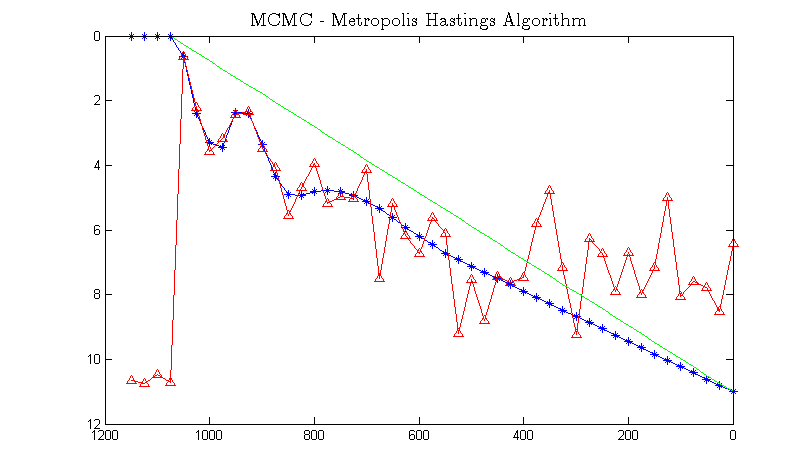
\includegraphics[width=5.5cm,height=3.8cm]{img/MCMC-manufactured_new.png}\\
       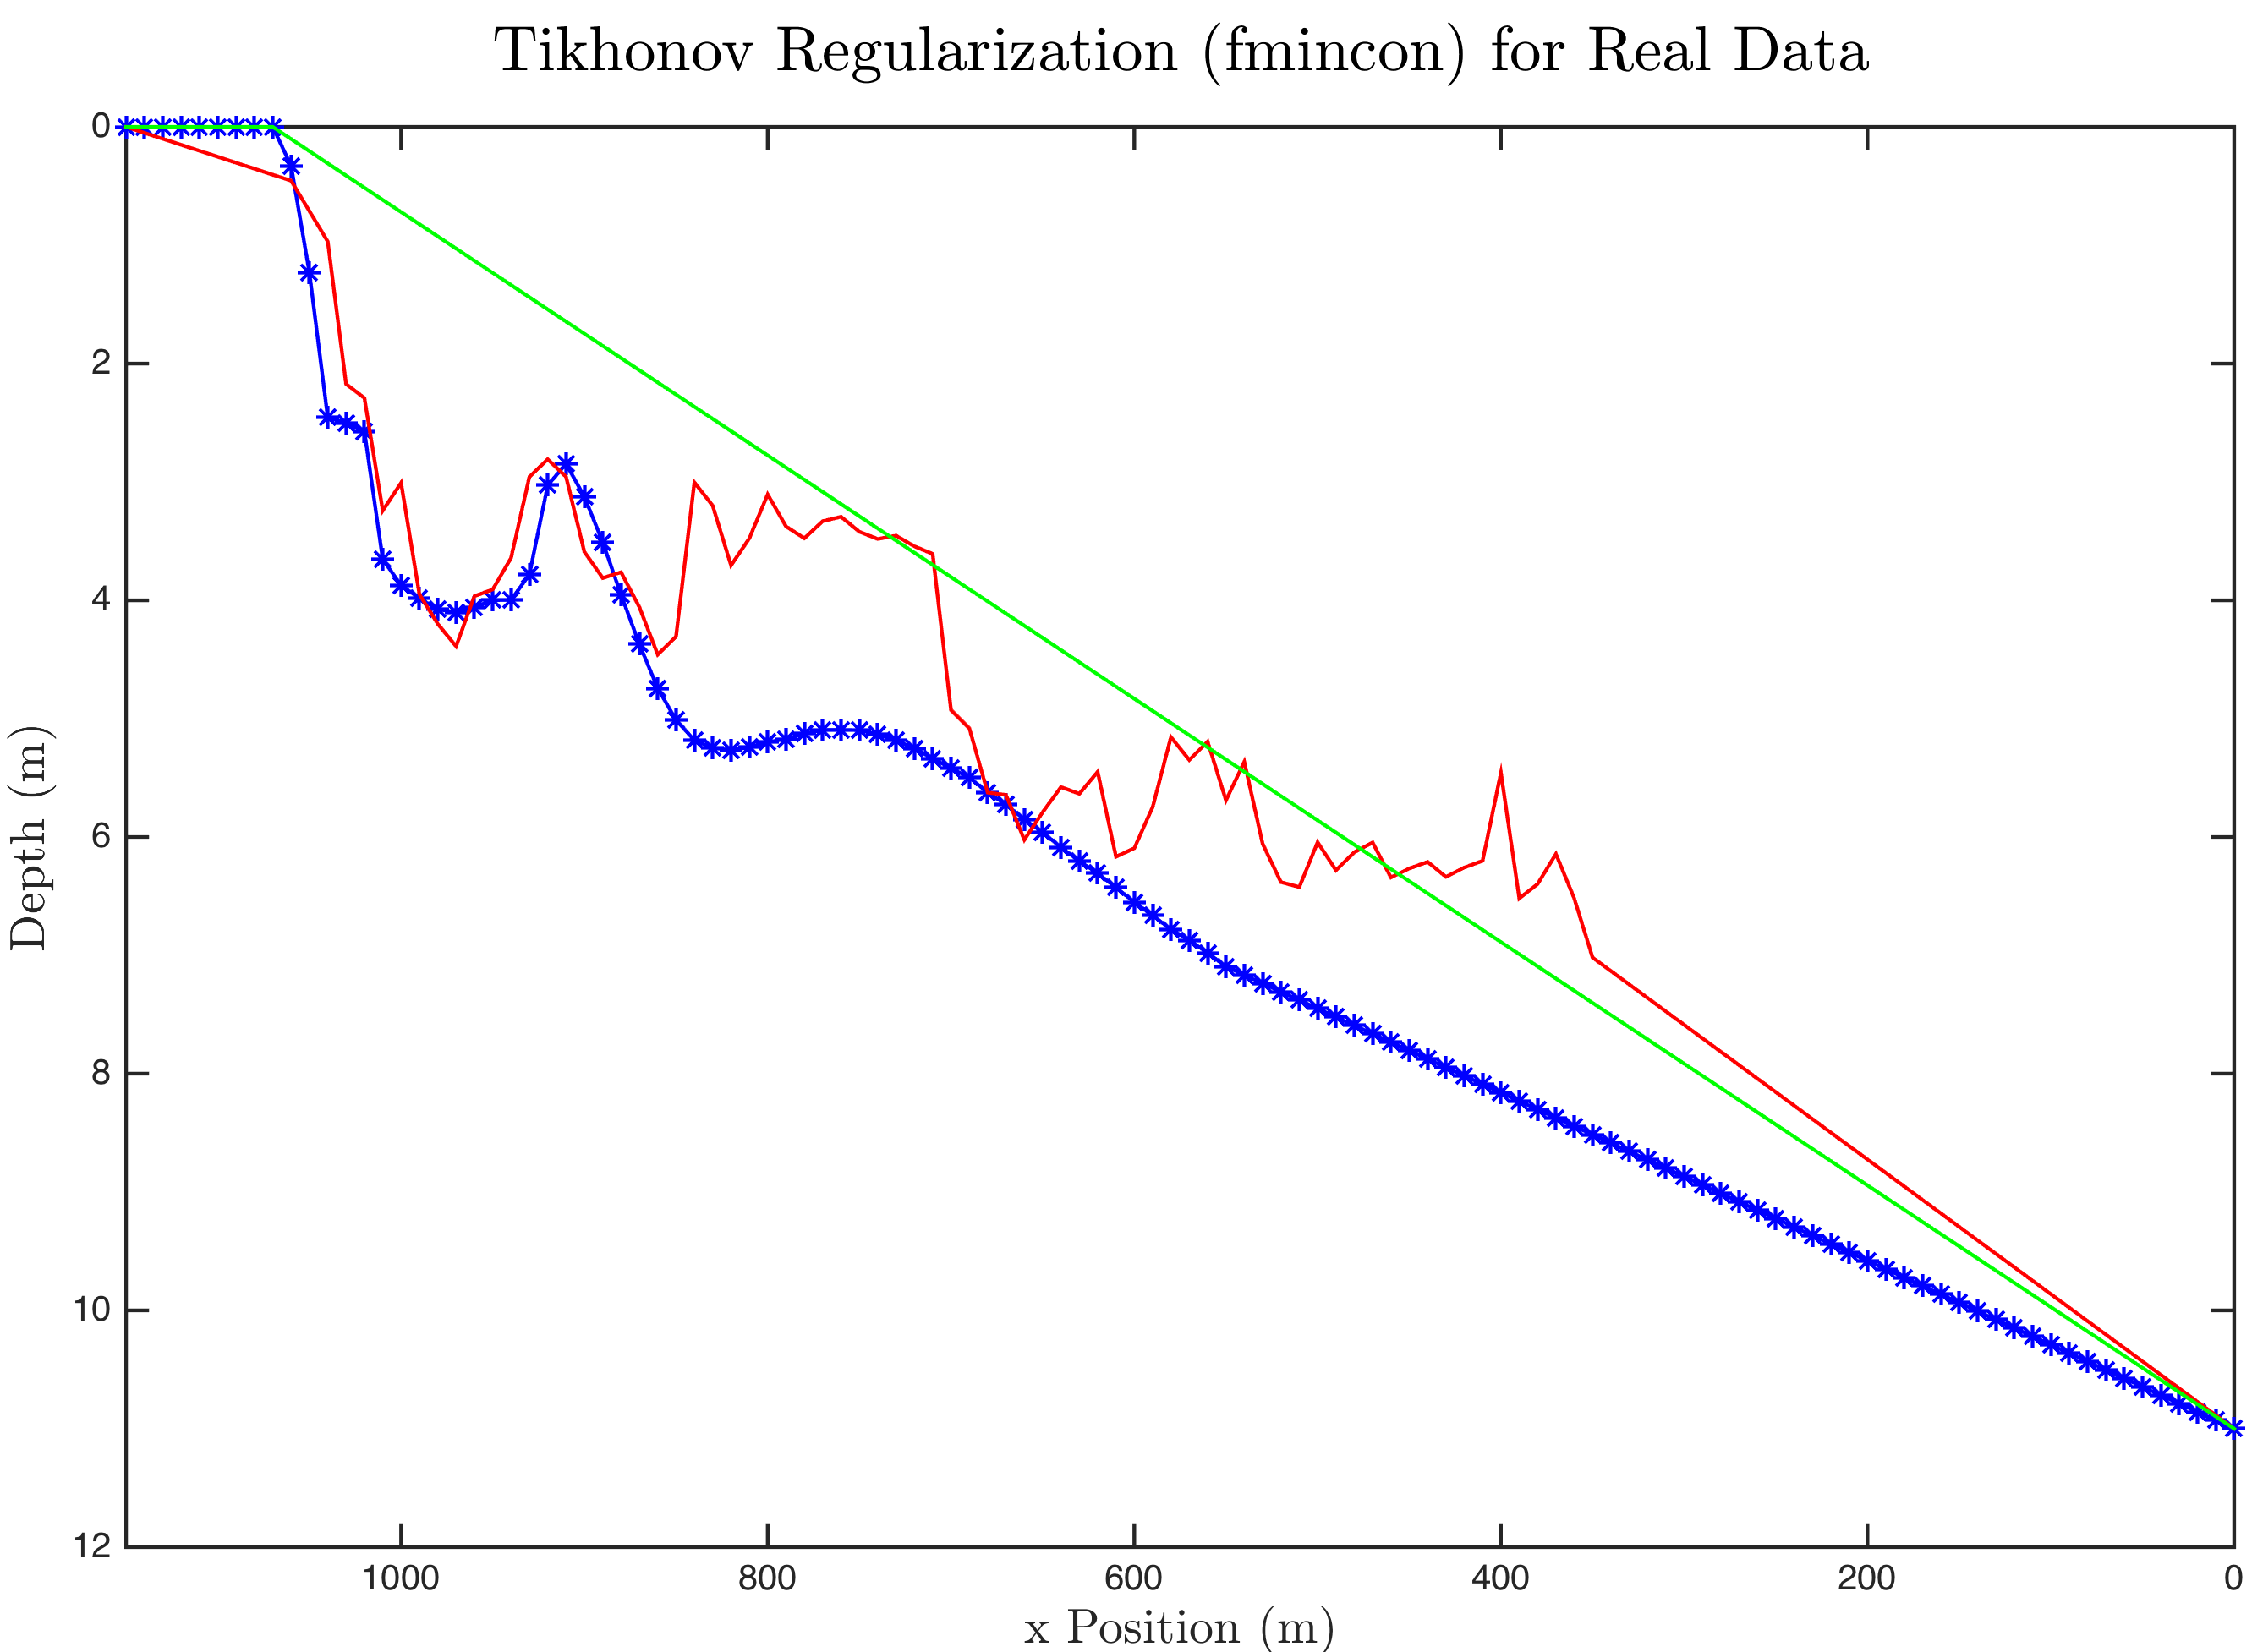
\includegraphics[width=4.8cm,height=3.5cm]{img/fmincon_real_data_oct09.png}
      \end{columns}
\end{frame}


%===================================================================================
% SLIDE 22
%===================================================================================
\begin{frame}
	\frametitle{Bathymetry estimates are limited by noisy $k$ data}
		\begin{figure}
			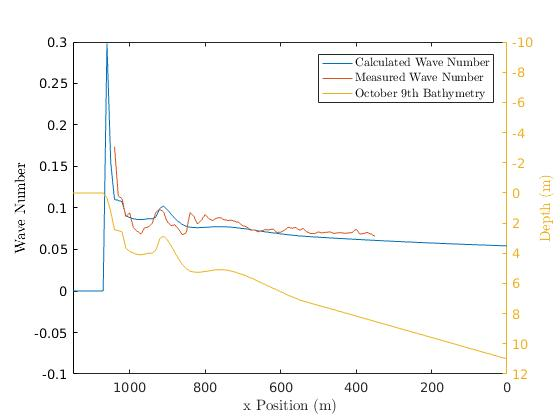
\includegraphics[width=1\linewidth]{img/Real_vs_Calcd_wavenum.jpg}
		\end{figure}
	
\end{frame}

%===================================================================================
% SLIDE 23
%===================================================================================
\begin{frame}
	\frametitle{Missing data \& deep water cause poor $h$ offshore}
		\begin{figure}[H]
			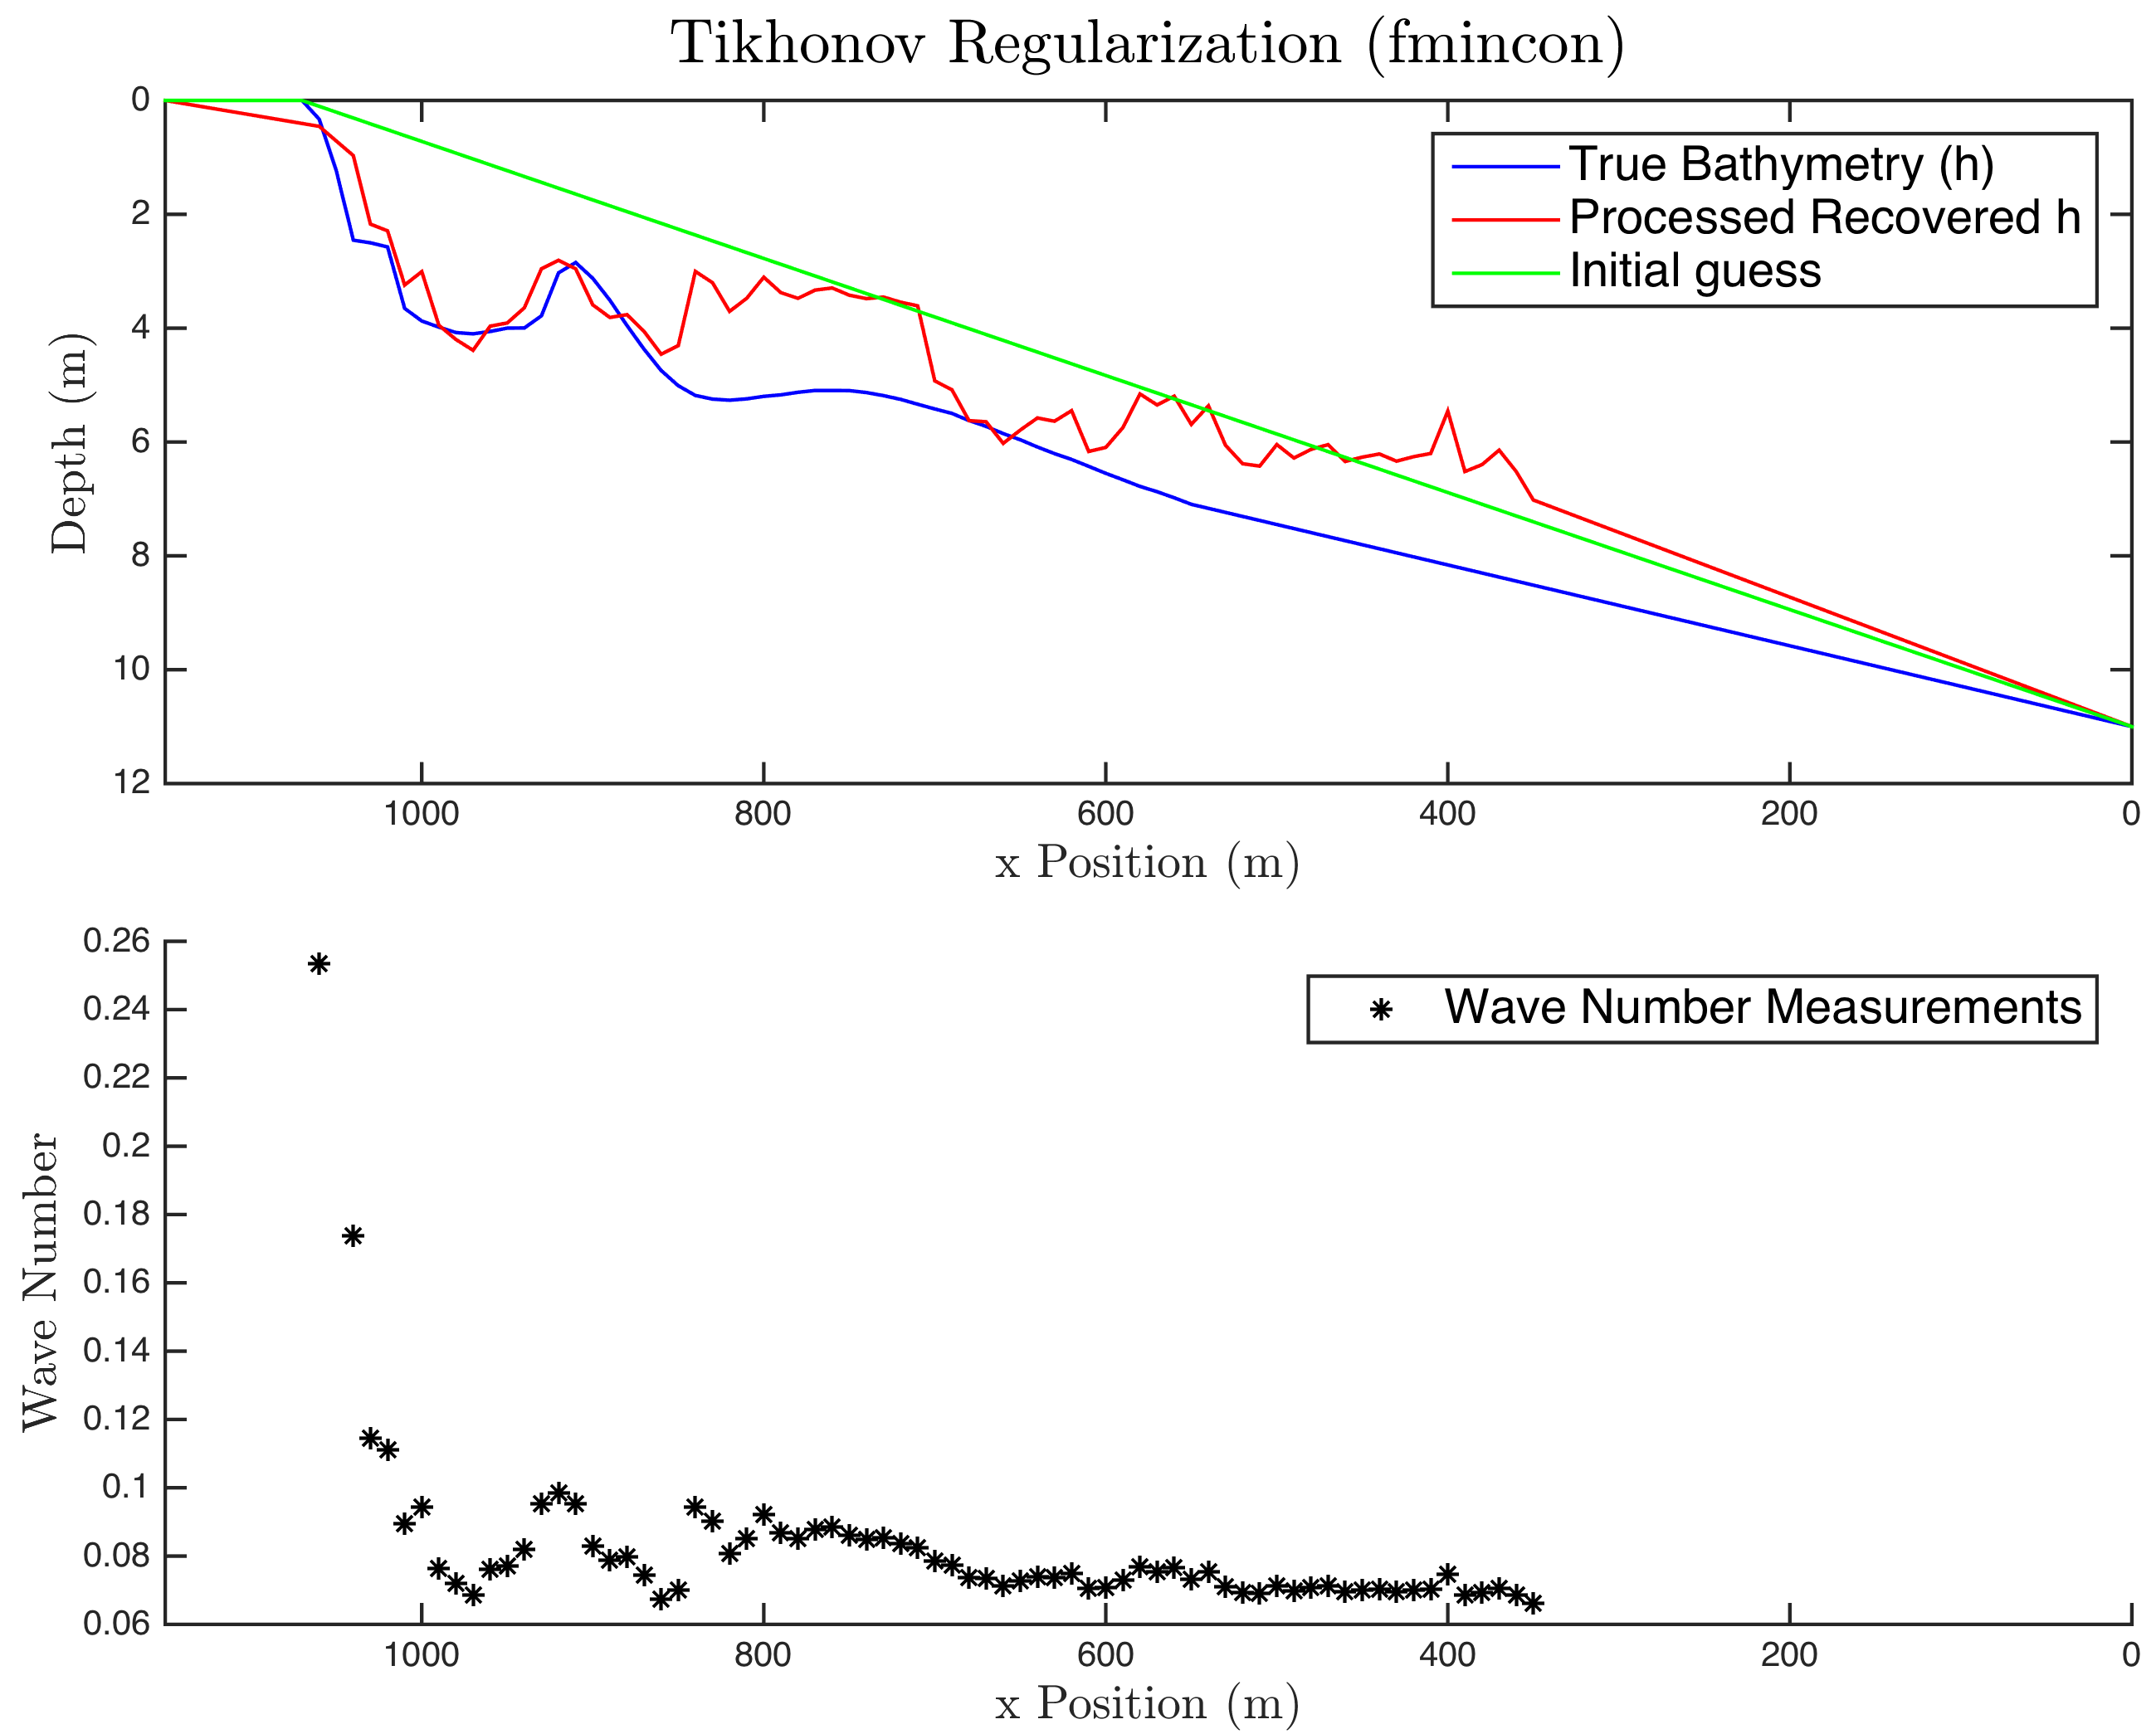
\includegraphics[width=0.9\linewidth]{img/fmincon_real_Oct09.png}
	 	\end{figure}
\end{frame}

%===================================================================================
%===================================================================================
\section{Discussion}
%===================================================================================
%===================================================================================

%===================================================================================
% SLIDE 24
%===================================================================================
\begin{frame}
	\frametitle{Future Directions}
		\begin{itemize}
			 \item Non-linear wave theory
			 	\begin{itemize}
				 	\item Linear wave theory is just a starting point!
			 	\end{itemize}
			 \item Inclusion of observed wave height, $H$, or other measured variables, along the profile
			 	\begin{itemize}
				 	\item this method will allow for assimilation of other measured variables
			 	\end{itemize}
			 \item Application of further regularization methods
			 	\begin{itemize}
				 	\item we heuristically ``tuned'' our regulariztion
				 	\item mayhaps incorporate prior knowledge?
			 	\end{itemize}
			 \item Incorporate uncertainty in measurements
			 \item Expansion to 2D wave physics
		\end{itemize}
\end{frame}

%===================================================================================
% Slide 25
%===================================================================================
\begin{frame}
	\frametitle{}
		\hspace{1.75cm}
		\begin{minipage}{70mm}   
                 	\begin{alertblock}{}    
                        		 \begin{center}
                  			\textbf{Thank you! \\Questions?}\\
		\begin{figure}[H]
			\includegraphics[width=0.6\linewidth]{img/Group_photo.jpg}
	 	\end{figure}
				\textbf{Acknowledgements:}\\
					NSF, USACE, SAMSI\\
					Anusha Madushani, Kimberly Kaufeld
				\end{center}
      			\end{alertblock}
		\end{minipage}
\end{frame}

%===================================================================================
% SLIDE 9: We tried several inverse methods
%===================================================================================

%\begin{frame}
% \frametitle{We tried several inverse methods}
%\begin{itemize}
%\item Nonlinear least squares
%\item MCMC
%\item fmincon
%\end{itemize}
%\end{frame}
%%==========================================================================================================================================
%
%%SLIDE 14: fmincon
%%==========================================================================================================================================
% \begin{frame}
%\frametitle{Additive Gaussian Noise Model}
%
%Gaussian noise $\boldsymbol{\epsilon}$ corrupted measurements $\mathbf{d}$ with variance $\nu$ is given by 
%$$
%\mathbf{d} = \mathbf{A} \mathbf{h}_t + \boldsymbol{\epsilon}.
%$$
%
%\begin{tabular}{l c l}
%$\mathbf{d}$ &=& a vector of measurements,\\
%$\mathbf{A}$ &=& a linear forward operator,\\
%$\mathbf{h}_t$ &=& the true bathymetry. 
%\end{tabular}
%
%\end{frame}
%
%
%%==========================================================================================================================================
%%SLIDE 15: fmincon
%%==========================================================================================================================================
% \begin{frame}
%\frametitle{fmincon: Tikhonov Method}
%\centering
%Uses a regularized solution with prior information
%$$
%\mathbf{\hat{h}} = \underset{\mathbf{h} \in \mathbb{R}^n}{\arg \min} \|  \mathbf{A}\mathbf{h} -  \mathbf{d} \|_2^2  +  \alpha \| \mathbf{h} -  \mathbf{h}_p\|_2^2,
%$$
%\end{frame}
%
%%==========================================================================================================================================
%% SLIDE 11: Bayesian Markov Chain Monte Carlo (MCMC) Method
%%======================================================================================
%
% \begin{frame}
%\frametitle{Bayesian Markov Chain Monte Carlo (MCMC) Method}
%The MCMC method creates a posterior distribution of depth profiles, given wave number by using the Bayes relationship
%
%\begin{equation}\label{bayes}
%P(h|%H,
%k) \propto \Pi(h)L(h|%H,
%k),
%\end{equation} 
%%\begin{itemize}
%%\item $\Pi(h)$  prior distribution
%%\item $L(h|%H,
%%k)$ likelihood function
%%\item $P(h|%H,
%%k)$ posterior distribution
%%\end{itemize}
%\end{frame}
%
%%==========================================================================================================================================
%% SLIDE 13: MCMC Method: Metropolis Algorithm
%%==========================================================================================================================================
%\begin{frame}
% \frametitle{MCMC Method: Metropolis Algorithm}
%\begin{itemize}
%\item Prior and likelihood are combined to compute an initial posterior probability distribution of \textit{h}\\
%\begin{equation}\label{post}
%P(h|%H,
%k) = log(\Pi(h)) + log(L(h|%H,
%k))
%\end{equation}
%\item Uses a markov chain random walk to %propose and compare new \textit{h} profiles
%arrive at a posterior distribution of \textit{h} profiles %which are expected to describe true bathymetry
%\end{itemize}
%\end{frame}
%%==========================================================================================================================================
%% SLIDE 10: Nonlinear least squares
%%===================================================================================================================
%
% \begin{frame}
%\frametitle{Nonlinear Least Squares: Trusted Region-Reflective Method}
%
%\begin{equation}\label{LS}
%\mathbf{\hat{h}}= \underset{\mathbf{h} \in \mathbb{R}^n}{\arg \min} \ \ f(\mathbf{h}) = \|  \mathbf{A}\mathbf{h} -  \mathbf{d} \|_2^2,
%\end{equation}
%
%\begin{figure}[H]
%	 	\centering
%	 	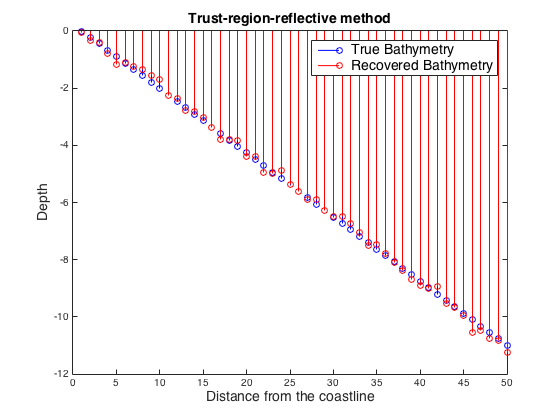
\includegraphics[width=.70\linewidth]{img/trust_region_linear.png}
%	 	\end{figure}
%
%\end{frame}
%
%
%%===========================================================================================================================================
%% SLIDE 12: MCMC Method: Log-Likelihood Function
%%======================================================================================
%\begin{frame}
% \frametitle{MCMC Method: Log-Likelihood Function}
% Loglikelihood function compares simulated and observed \textit{k}
%
%\begin{equation} \label{likely}
%\log{L(h|%H,
%k)}=log[{exp(- \frac{\sum\limits_{i=1}^n({k}_{m,i}-k_{d,i})^2}{2\sigma_{k}^2})]}
%\end{equation} 
%
%
%\end{frame}
%%==========================================================================================================================================
%

\end{document}
>>>>>>> c5866c7ef909ec56d6a3f233480b14eea86baa38


    %====================================================================================
    % SLIDE 11
    %====================================================================================
    \begin{frame}
      \frametitle{Data includes $T$, $H$ at offshore boundary; 1D $k$}
      \begin{figure}[H]
        \centering
        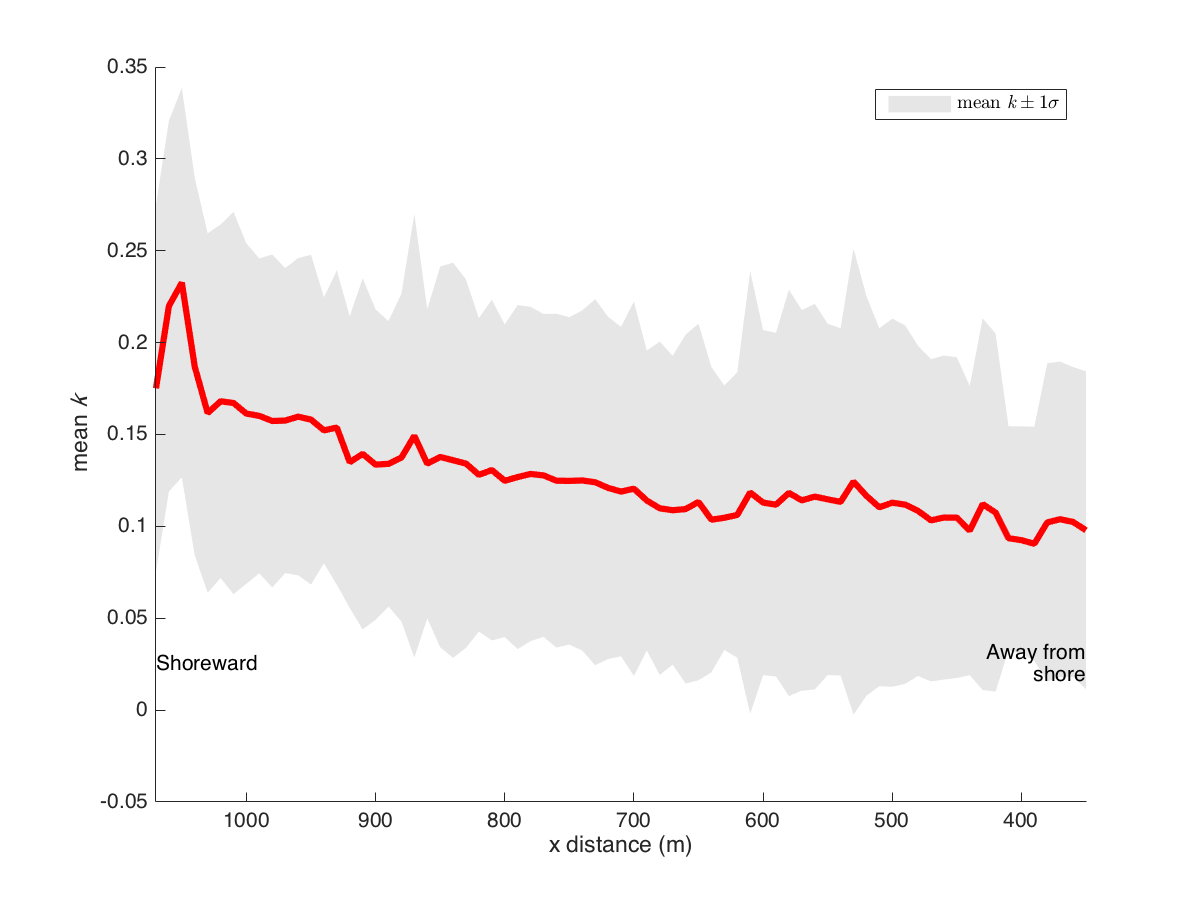
\includegraphics[width=1\linewidth]{img/k1Dmean_std.png}
      \end{figure}
    \end{frame}

    %====================================================================================
    % SLIDE 12
    %====================================================================================
    \begin{frame}
      \frametitle{Known bathymetry is used for testing our results}
      %\begin{columns}
      %\column{0.5\textwidth}
      \begin{figure}[H]
        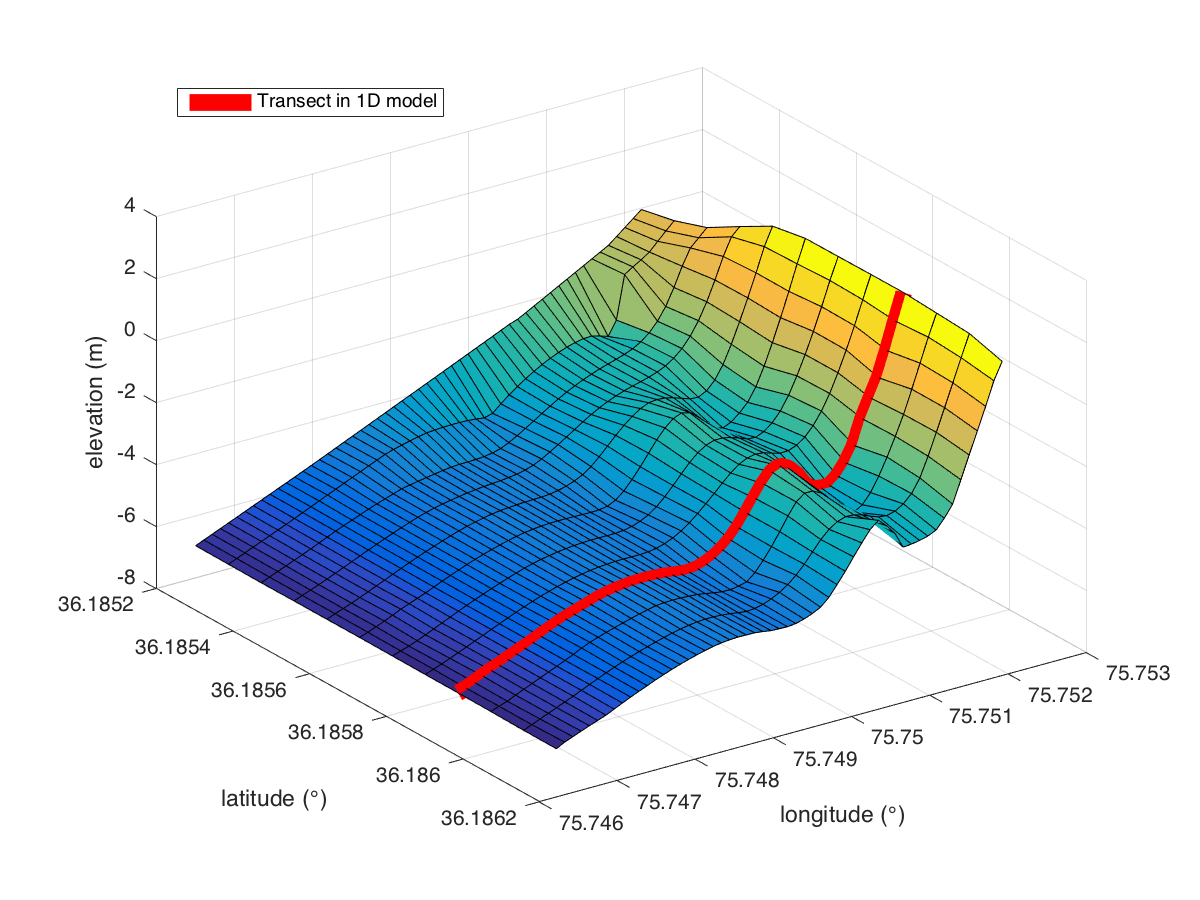
\includegraphics[width=1\linewidth]{img/trueBath2D.png}
      \end{figure}
      %\column{0.5\textwidth}
      %\begin{figure}[h]
      %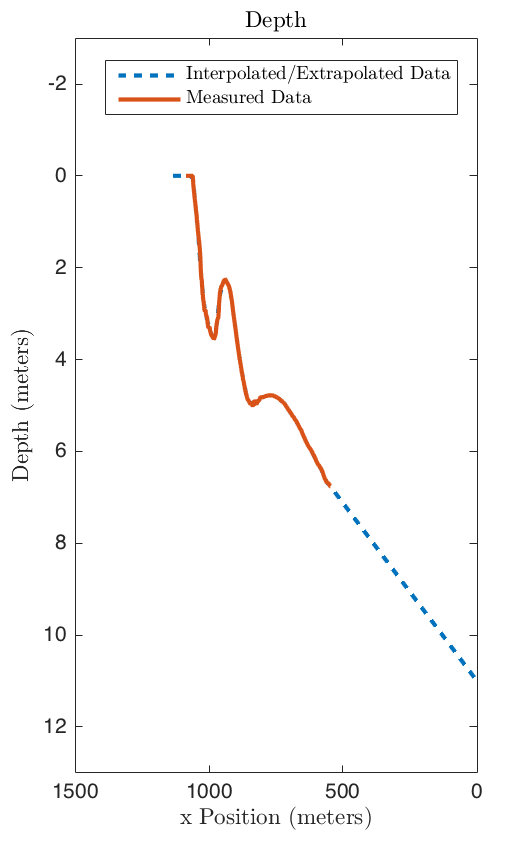
\includegraphics[width=.70\linewidth]{img/DepthChart.png}
      %\end{figure}
      %\end{columns}
    \end{frame}

    %==================================================================================
    %==================================================================================
    \section{Forward Model}
    %==================================================================================
    %==================================================================================

    %==================================================================================
    % SLIDE 13
    %==================================================================================
    \begin{frame}
      \frametitle{Forward model computes $k$ assuming $h_{guess}$ \& BC}
      \begin{figure}[H]
        \centering
        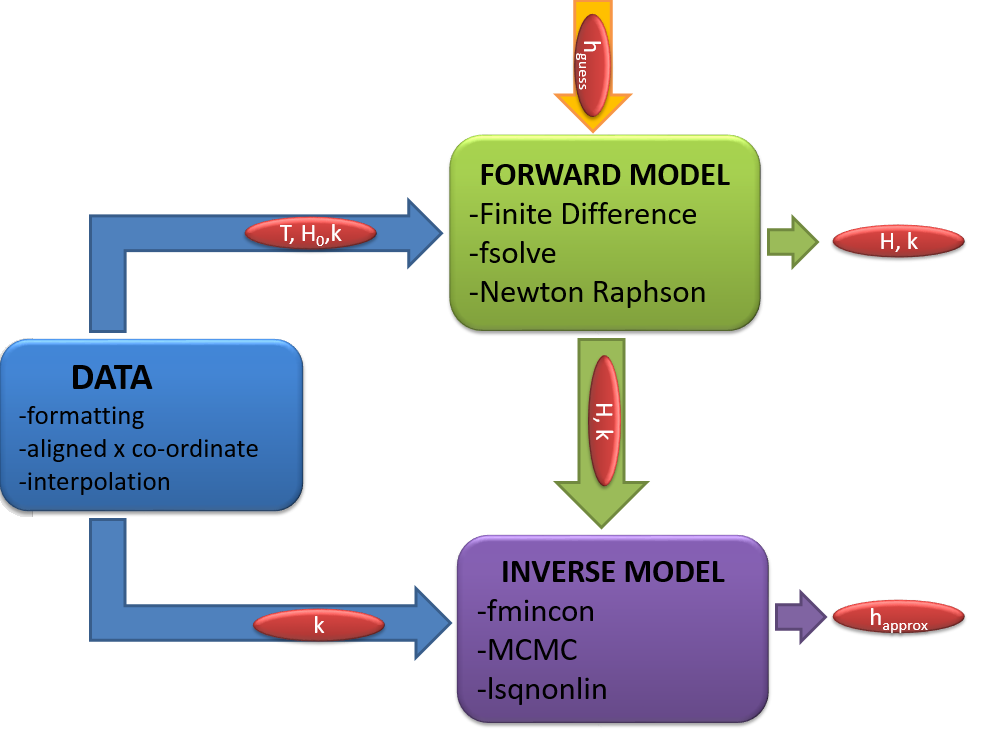
\includegraphics[width=1.0\linewidth]{img/Flow_New.png}
      \end{figure}
    \end{frame}

    %==================================================================================
    % SLIDE 14
    %==================================================================================
    \begin{frame}
      \frametitle{Wave dispersion relationship relates $k$ to $h$}
      Dispersion Relation:
      $$ \sigma^2=gk\tanh(kh) \Longleftrightarrow \left(\frac{2\pi}{T}\right)^2 = g\left(\frac{2\pi}{L}\right) tanh \left(\frac{2\pi h}{L}\right)
      $$
      \begin{itemize}
      \item Relates wave number $(k)$ and Period $(T)$
      \item Wave length $(L)$ varies with depth $(h)$
      \item Period $(T)$ remains constant
      \end{itemize}
    \end{frame}


    %==================================================================================
    % SLIDE 15
    %==================================================================================
    \begin{frame}
      \frametitle{1D forward model relates $H$ and $h$}
      Energy Flux Method:
      $$\frac{d}{dx}\left(EC_g\right)=-\delta $$
      %\begin{itemize}
      \centering
      $\delta = \frac{1}{4h}B\rho g f H^3_{rms}\left[(R^3+\frac{3}{2}R)e^{-R^2}+\frac{3}{4}\sqrt{\pi}(1-erf(R))\right]$
      (Janssen and Battjes, 2007) \\
      %\end{itemize} \\
      $\,$\\
      where $R=\frac{H_b}{H_{rms}}$, $H_b=0.78h$, $H_{rms}=0.7H$. \\
      $\,$\\
      \begin{itemize}
      \item $E$: Wave Energy $(\rho,g,H)$
      \item  $C_{g}$: Group celerity $(\sigma,k,h)$
      \end{itemize}
    \end{frame}

    %==================================================================================
    %==================================================================================
    \section{Inverse Methods}
    %==================================================================================
    %==================================================================================

    %==================================================================================
    % SLIDE 16
    %==================================================================================
    \begin{frame}
      \frametitle{Invert for bathymetry given surface data \& physics}
      \begin{figure}
        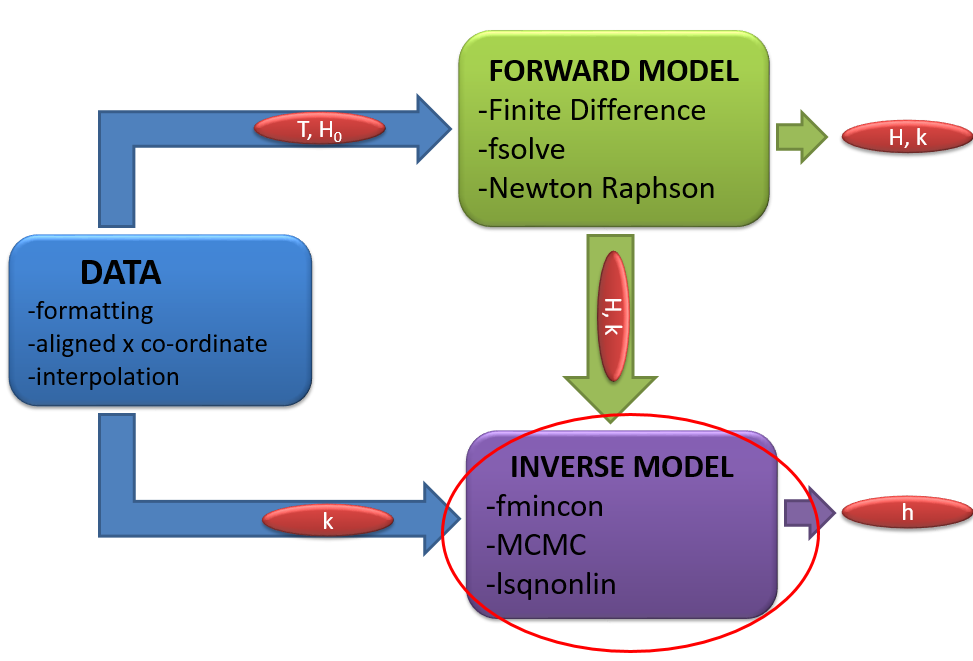
\includegraphics[width=1.0\linewidth]{img/INV.png}
      \end{figure}
    \end{frame}

    %==================================================================================
    % SLIDE 17
    %==================================================================================
    \begin{frame}
      \frametitle{Solutions are computed using 3 inversion methods}
      \centering
      \begin{enumerate}
      \item Nonlinear Least Squares (lsqnonlin)
        \begin{itemize}
        \item Logical place to start
        \end{itemize}
        $\,$\\
      \item Bayesian MCMC (Metropolis)
        \begin{itemize}
        \item Gives a distribution of depth estimates
        \end{itemize}
        $\,$\\
      \item Tikhonov Regularization (fmincon)
        \begin{itemize}
        \item Bounded-constraint multivariate problem
        \end{itemize}
      \end{enumerate}
    \end{frame}

    %==================================================================================
    \subsection{Manufactured}
    %==================================================================================

    %==================================================================================
    %  SLIDE 18
    %==================================================================================
    \begin{frame}
      \frametitle{Manufactured ``data'' is used to test our algorithms}
      \begin{figure}
        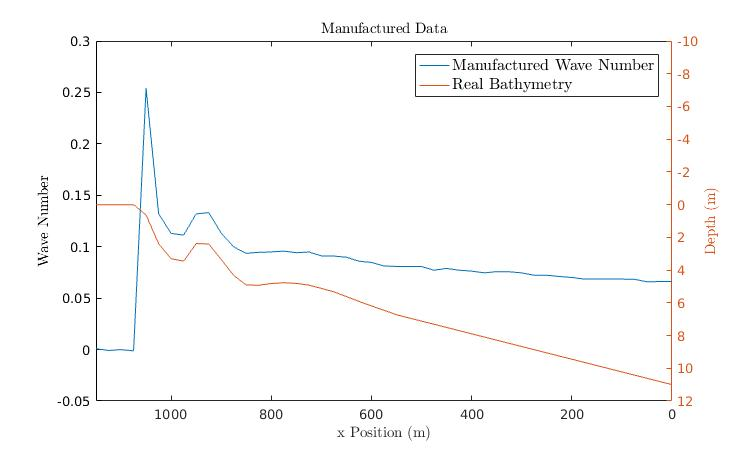
\includegraphics[width=1.0\linewidth]{img/Manufactured_data.jpg}
      \end{figure}
    \end{frame}


    %==================================================================================
    %  SLIDE 19
    %==================================================================================
    \begin{frame}
      \frametitle{All methods capture the sandbar well}
      \begin{columns}
        %          \column{0.5\textwidth}
        %\begin{figure}[H]
        % \centering
        %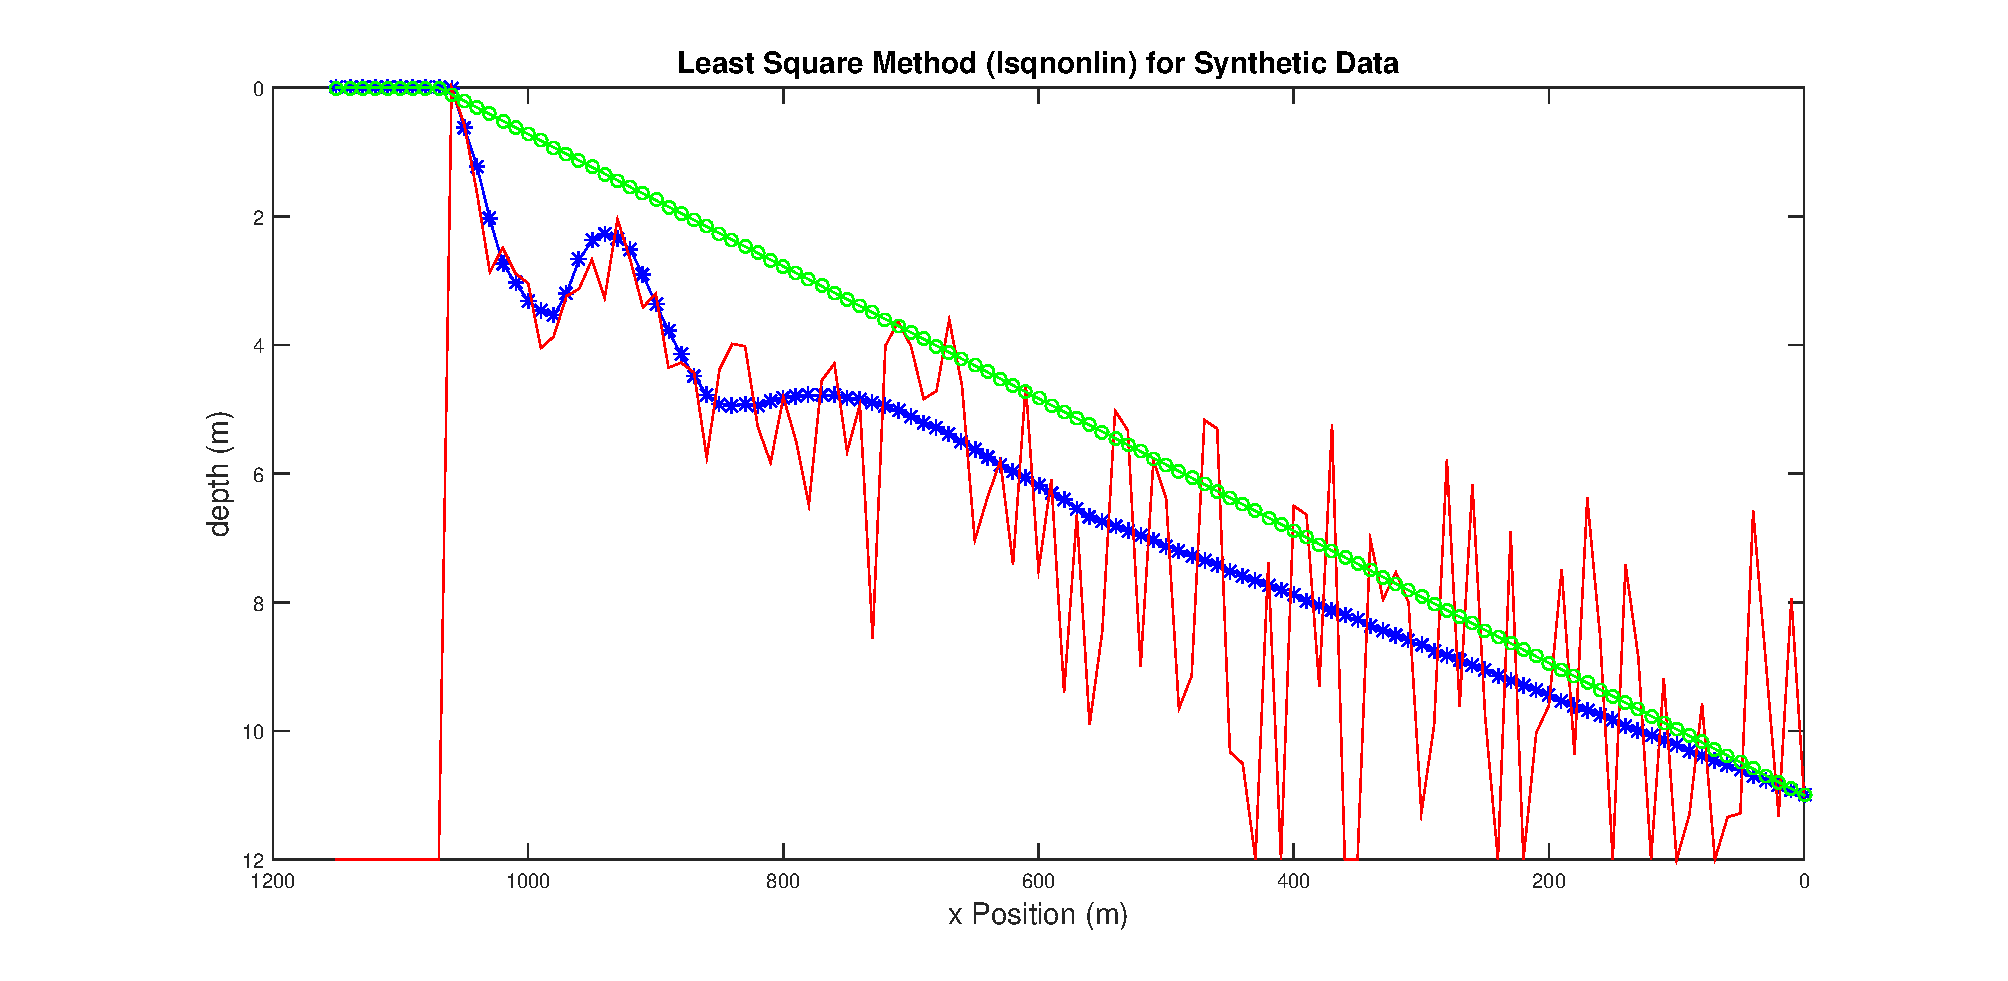
\includegraphics[width=0.5\linewidth]{img/lsqnonlin_simulated_10m_new.eps}
        %\end{figure}
        %\column{0.5\textwidth}
        %\begin{figure}[H]
        % 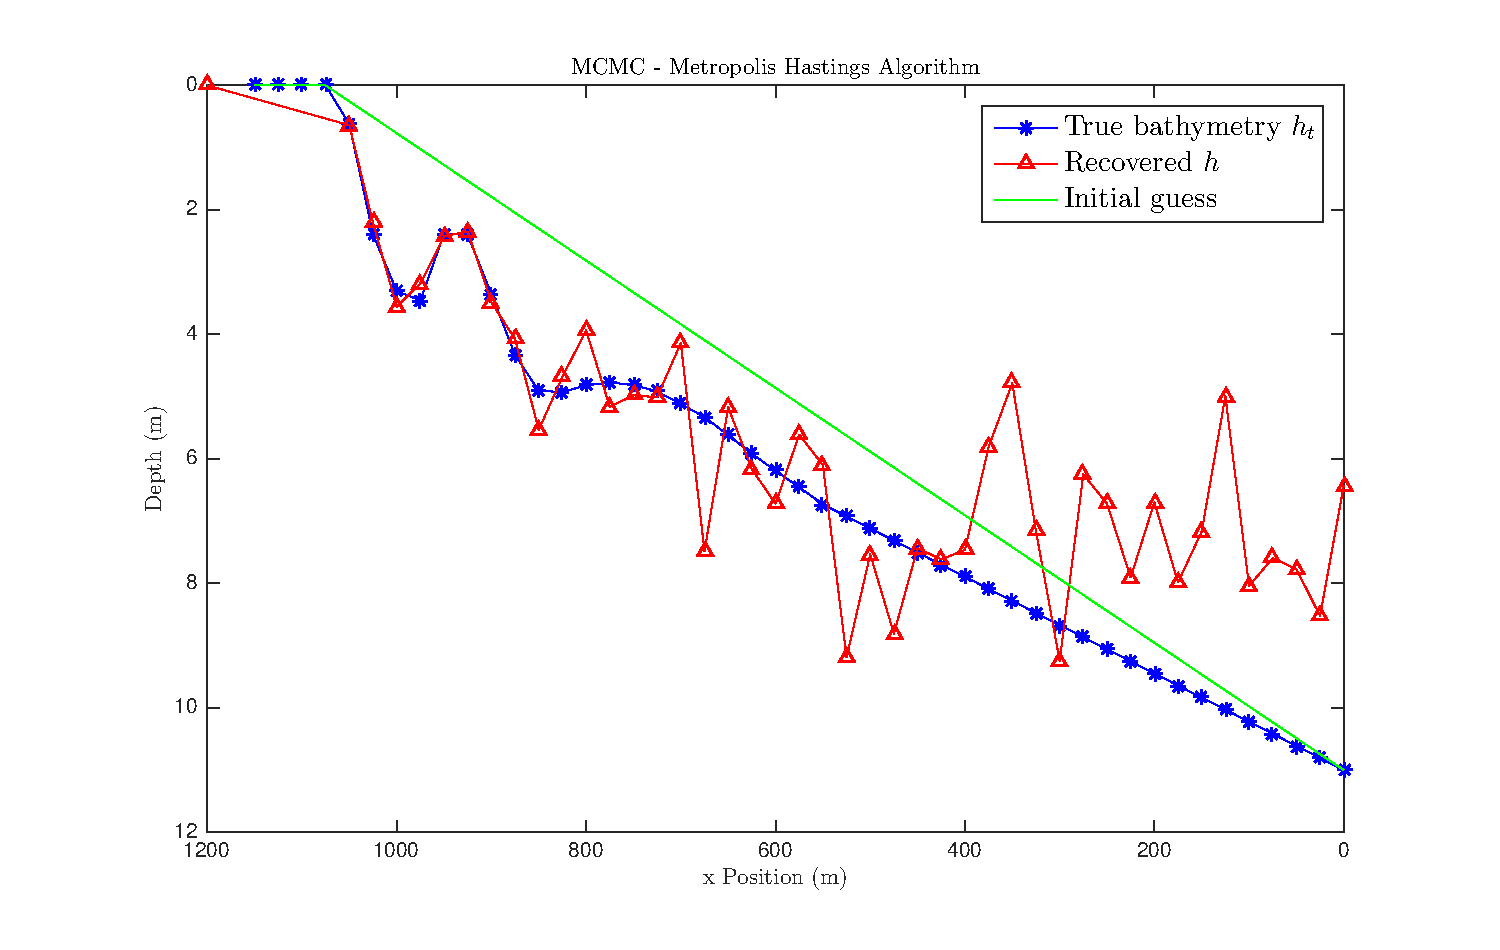
\includegraphics[width=1\linewidth]{img/MCMC-manufactured.eps}\vfill
        %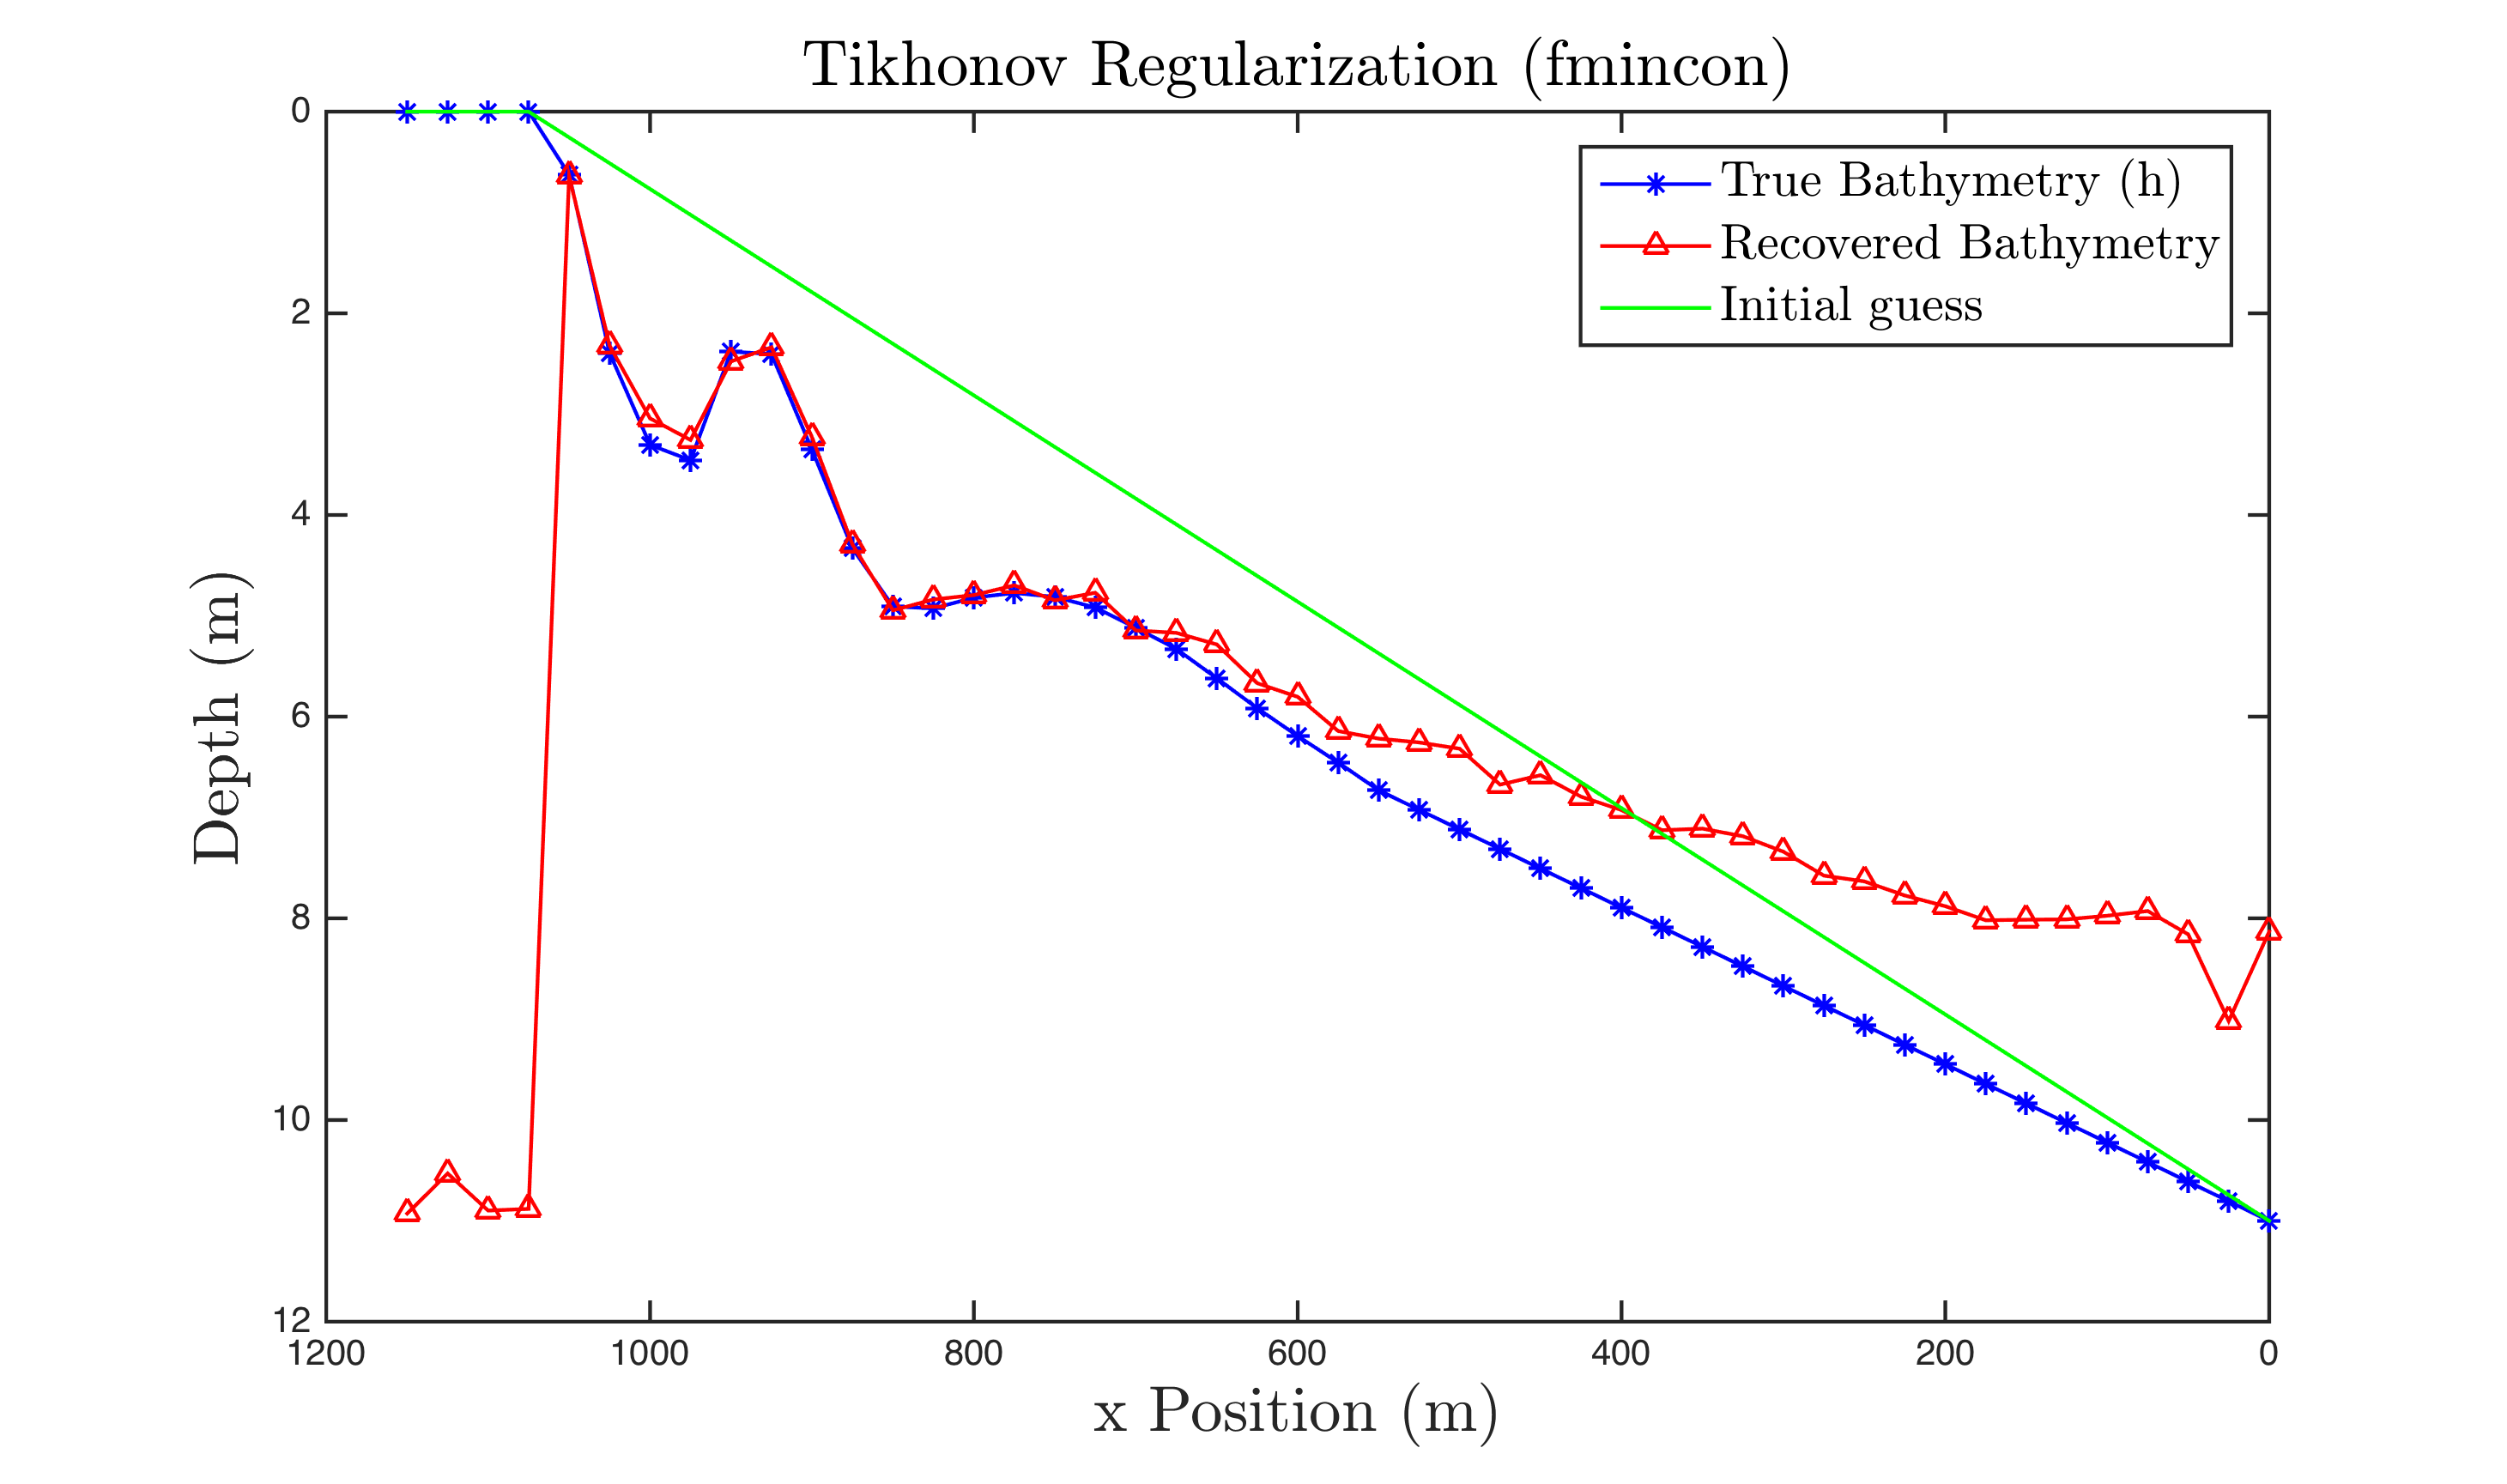
\includegraphics[width=1\linewidth]{img/fmincon_simulated_25m.png}
        % \end{figure}
      \end{columns}
    \end{frame}

    %==================================================================================
    \subsection{Real}
    %==================================================================================

    %===================================================================================
    % SLIDE 20
    %===================================================================================
    \begin{frame}
      \frametitle{Real $k$ data is selected for a period with low noise}
      \begin{figure}
        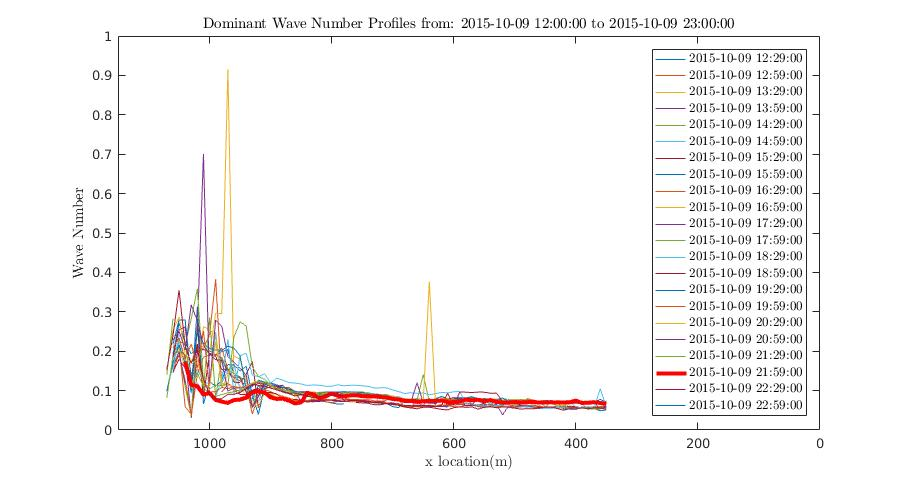
\includegraphics[width=1.0\linewidth]{img/Real_k_data.jpg}
      \end{figure}
    \end{frame}


    %===================================================================================
    % SLIDE 21
    %===================================================================================
    \begin{frame}
      \frametitle{Bathymetry estimates perform well in shallow water}
      %\begin{columns}
      %          \column{0.5\textwidth}
      %\begin{figure}[H]
      % \centering
      %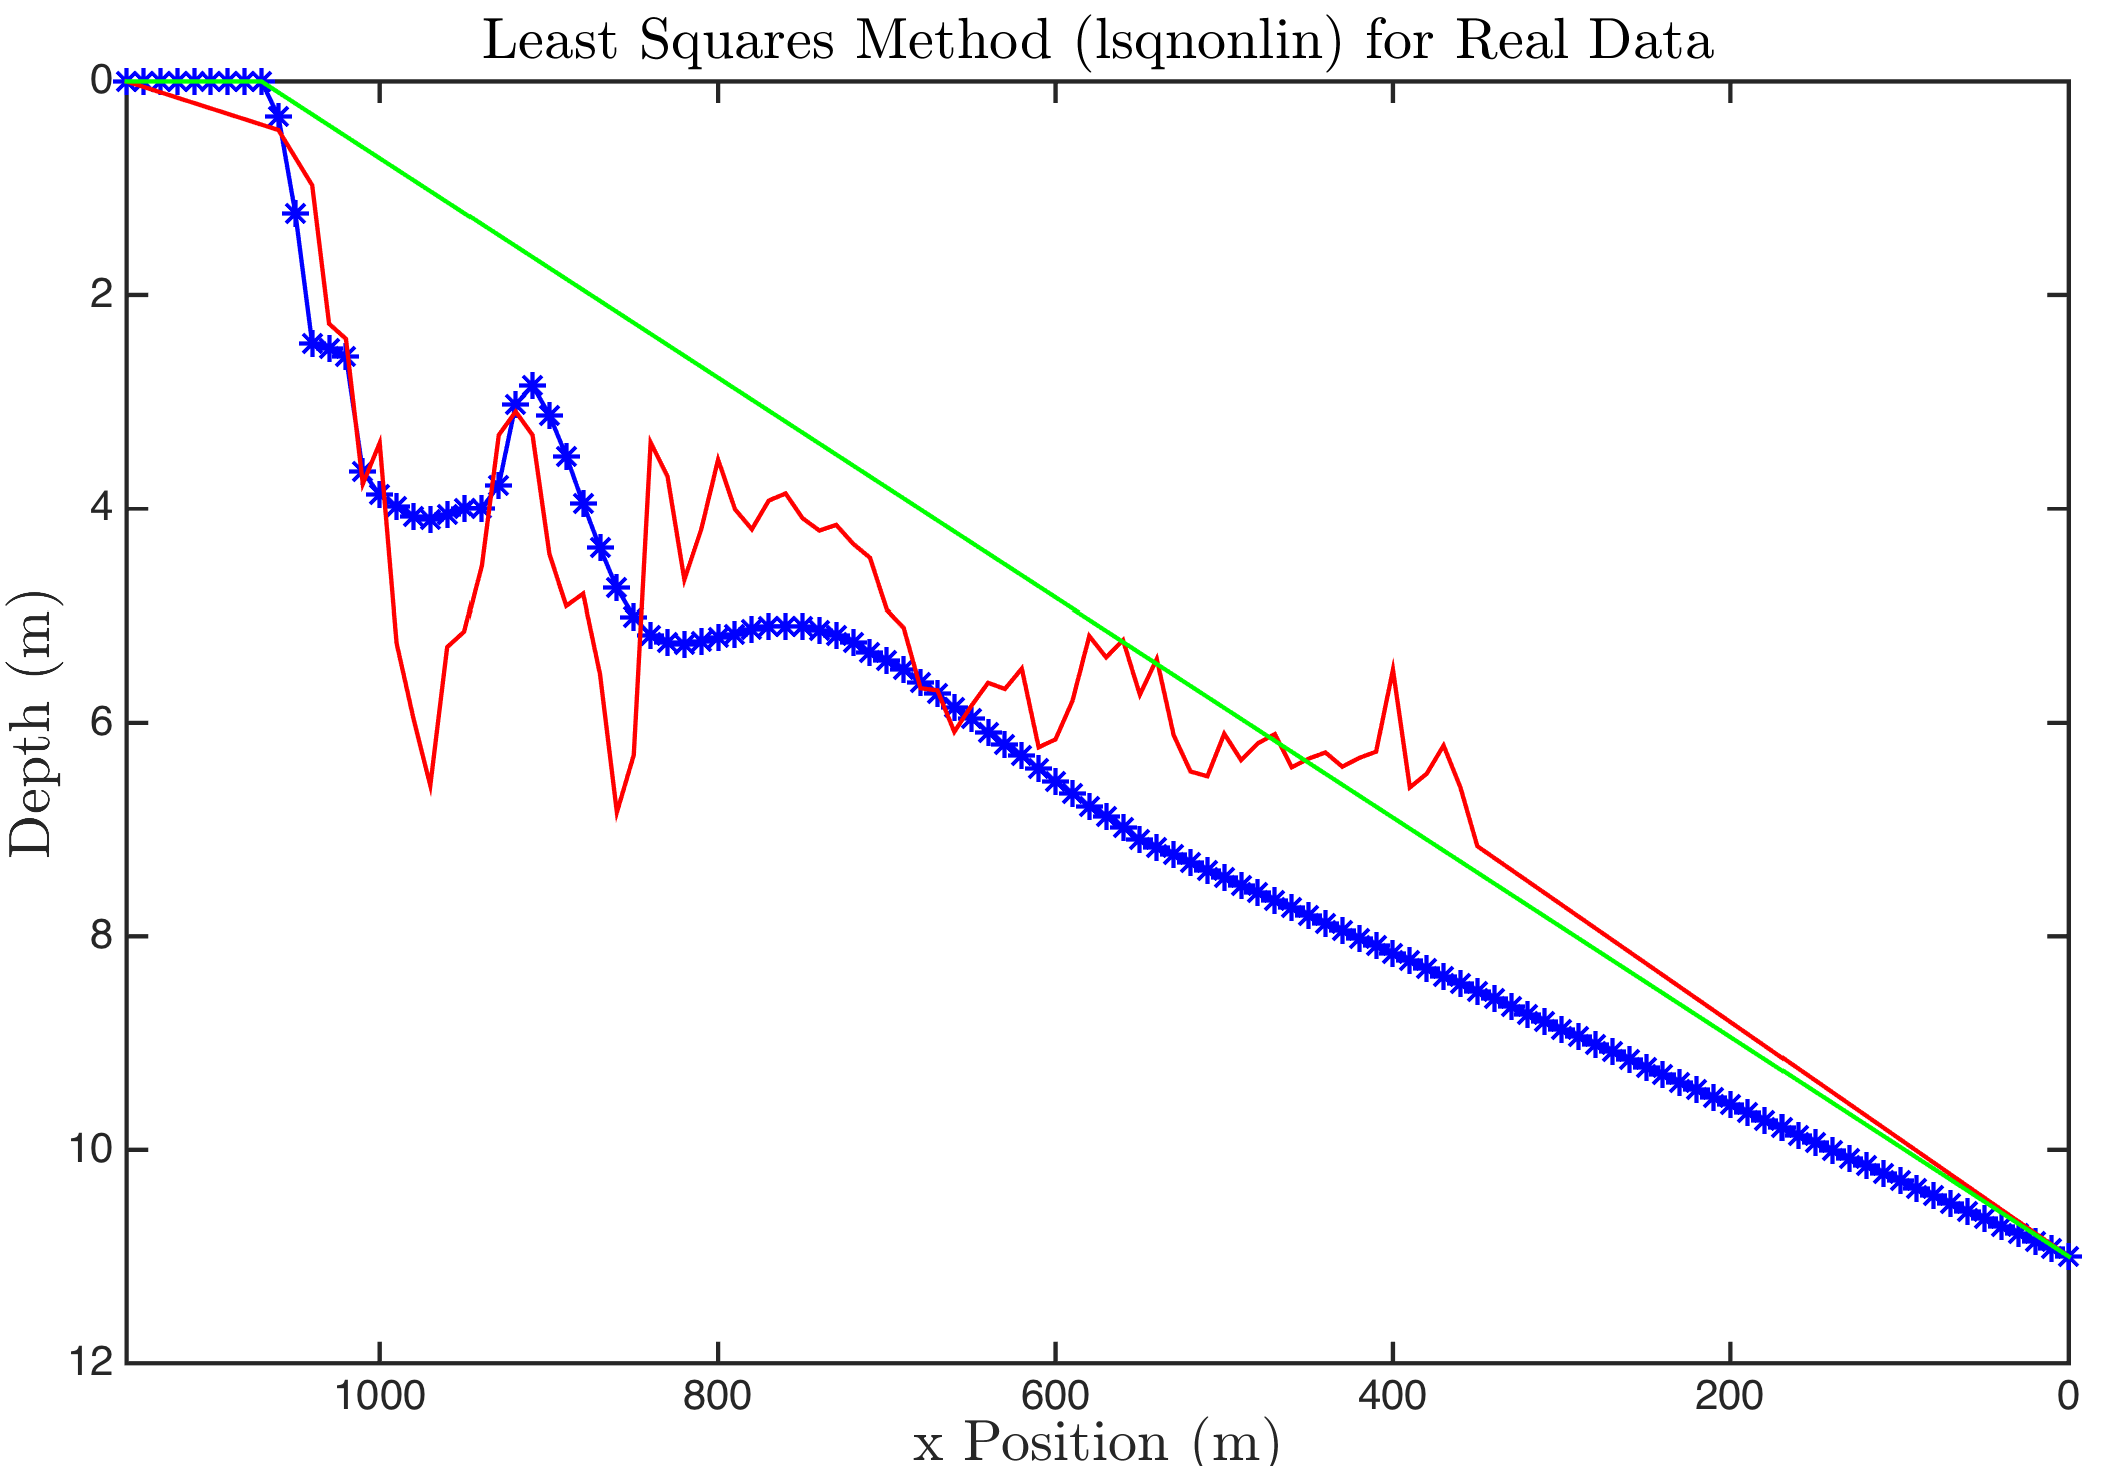
\includegraphics[width=1\linewidth]{img/lsqnonlin_real_data_oct09}
      %\end{figure}
      %\column{0.5\textwidth}
      %\begin{figure}[H]
      % 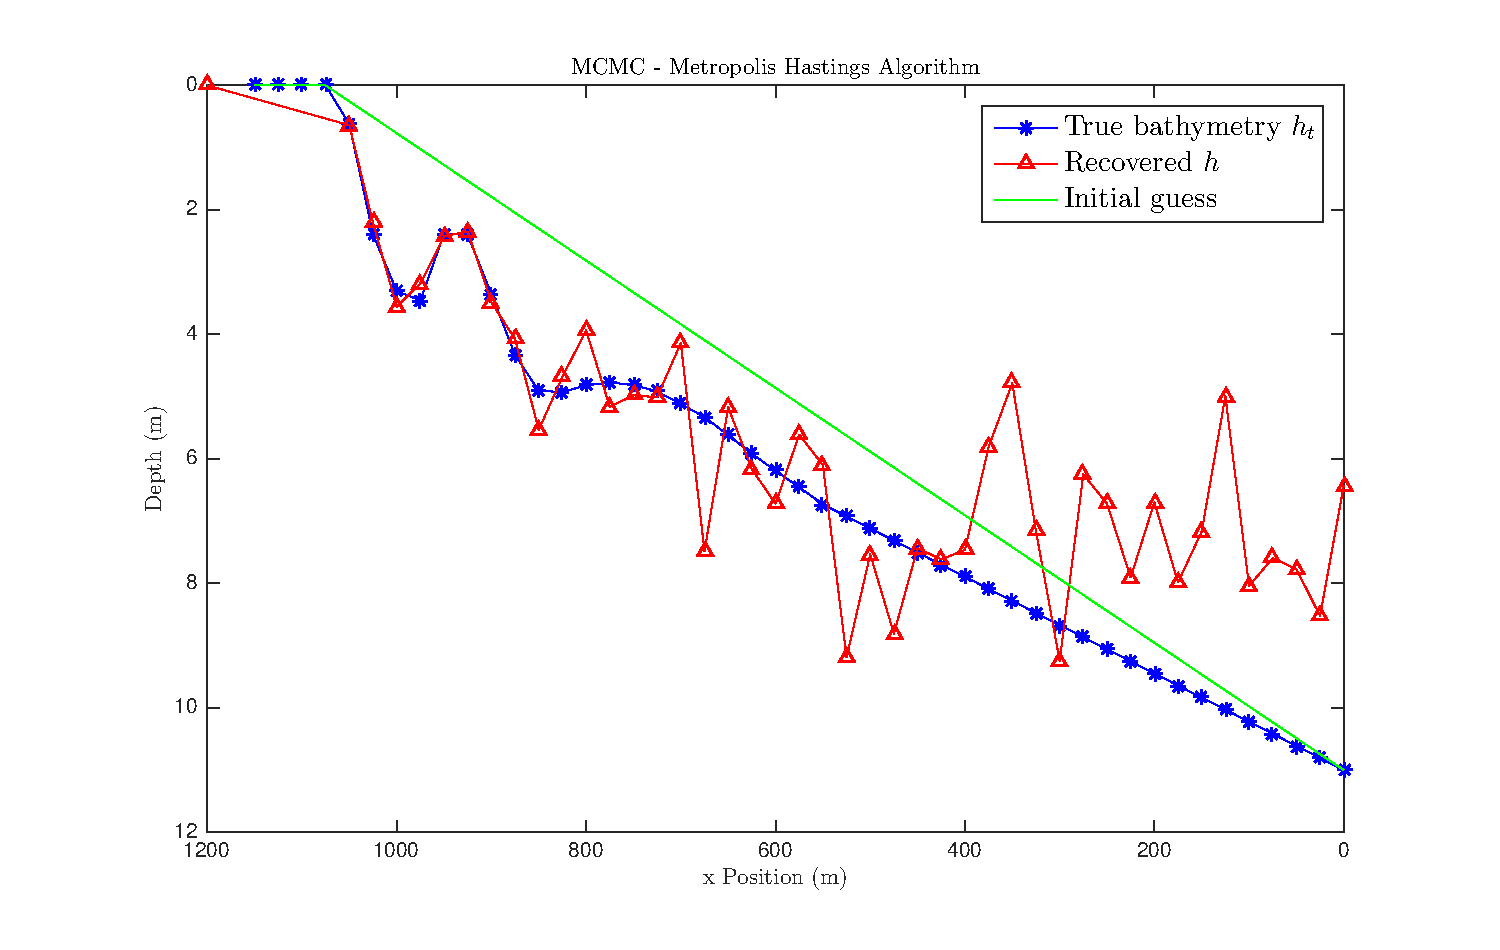
\includegraphics[width=1\linewidth]{img/MCMC-manufactured.eps}\vfill
      %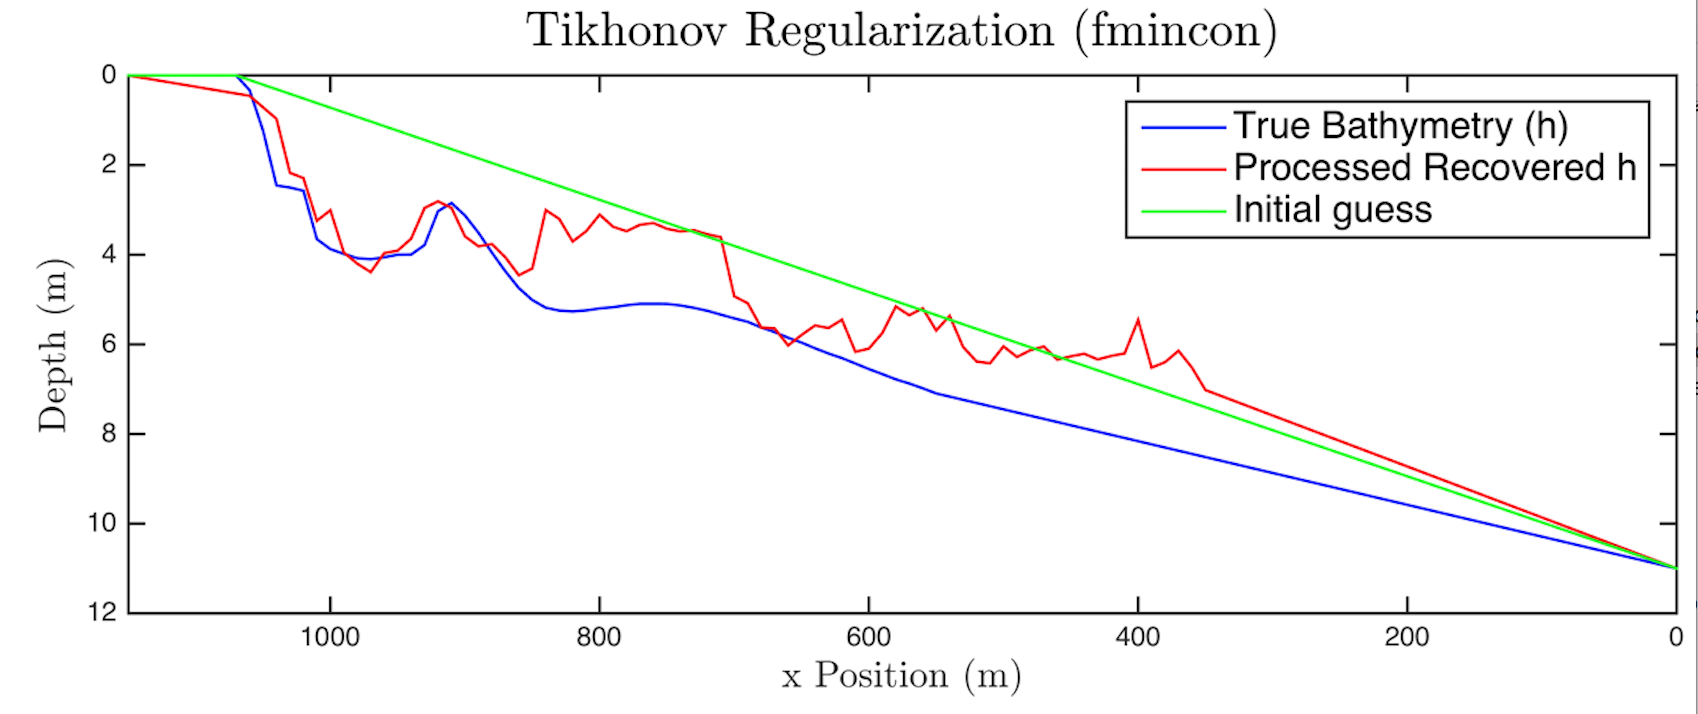
\includegraphics[width=1\linewidth]{img/fmincon_real_Oct09_nok.png}
      % \end{figure}
      %\end{columns}
    \end{frame}

    %===================================================================================
    % SLIDE 22
    %===================================================================================
    \begin{frame}
      \frametitle{Bathymetry estimates are limited by noisy $k$ data}
      \begin{figure}
        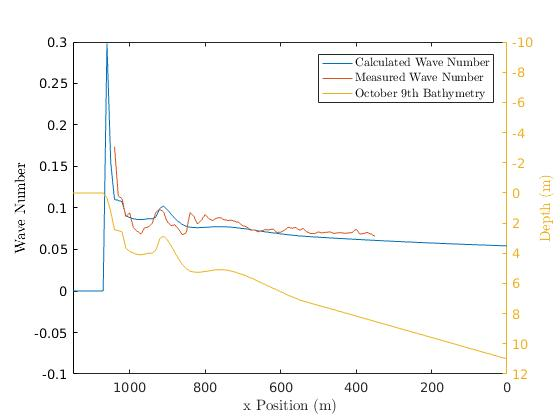
\includegraphics[width=1\linewidth]{img/Real_vs_Calcd_wavenum.jpg}
      \end{figure}

    \end{frame}

    %===================================================================================
    % SLIDE 23
    %===================================================================================
    \begin{frame}
      \frametitle{Missing data \& deep water cause poor $h$ offshore}
      \begin{figure}[H]
        \includegraphics[width=0.9\linewidth]{img/fmincon_real_Oct09.png}
      \end{figure}
    \end{frame}

    %===================================================================================
    %===================================================================================
    \section{Discussion}
    %===================================================================================
    %===================================================================================

    %===================================================================================
    % SLIDE 24
    %===================================================================================
    \begin{frame}
      \frametitle{Future Directions}
      \begin{itemize}
      \item Non-linear wave theory
        \begin{itemize}
        \item Linear wave theory is just a starting point!
        \end{itemize}
      \item Inclusion of observed wave height, $H$, or other measured variables, along the profile
        \begin{itemize}
        \item this method will allow for assimilation of other measured variables
        \end{itemize}
      \item Application of further regularization methods
        \begin{itemize}
        \item we heuristically ``tuned'' our regulariztion
        \item mayhaps incorporate prior knowledge?
        \end{itemize}
      \item Incorporate uncertainty in measurements
      \item Expansion to 2D wave physics
      \end{itemize}
    \end{frame}

    %===================================================================================
    % Slide 25
    %===================================================================================
    \begin{frame}
      \frametitle{}
      \hspace{2.5cm}
      \begin{minipage}{50mm}
        \begin{alertblock}{}
          \begin{center}
            \textbf{Thank you! \\Questions?}\\
            $\,$\\
            $\,$\\
            \textbf{Acknowledgements:}\\
            NSF\\
            USACE\\
            SAMSI\\
            Anusha Madushani\\
            Kimberly Kaufeld
          \end{center}
        \end{alertblock}
      \end{minipage}
    \end{frame}

    %===================================================================================
    % SLIDE 9: We tried several inverse methods
    %===================================================================================

    %\begin{frame}
    % \frametitle{We tried several inverse methods}
    %\begin{itemize}
    %\item Nonlinear least squares
    %\item MCMC
    %\item fmincon
    %\end{itemize}
    %\end{frame}
    %%==========================================================================================================================================
    %
    %%SLIDE 14: fmincon
    %%==========================================================================================================================================
    % \begin{frame}
    %\frametitle{Additive Gaussian Noise Model}
    %
    %Gaussian noise $\boldsymbol{\epsilon}$ corrupted measurements $\mathbf{d}$ with variance $\nu$ is given by
    %$$
    %\mathbf{d} = \mathbf{A} \mathbf{h}_t + \boldsymbol{\epsilon}.
    %$$
    %
    %\begin{tabular}{l c l}
    %$\mathbf{d}$ &=& a vector of measurements,\\
    %$\mathbf{A}$ &=& a linear forward operator,\\
    %$\mathbf{h}_t$ &=& the true bathymetry.
    %\end{tabular}
    %
    %\end{frame}
    %
    %
    %%==========================================================================================================================================
    %%SLIDE 15: fmincon
    %%==========================================================================================================================================
    % \begin{frame}
    %\frametitle{fmincon: Tikhonov Method}
    %\centering
    %Uses a regularized solution with prior information
    %$$
    %\mathbf{\hat{h}} = \underset{\mathbf{h} \in \mathbb{R}^n}{\arg \min} \|  \mathbf{A}\mathbf{h} -  \mathbf{d} \|_2^2  +  \alpha \| \mathbf{h} -  \mathbf{h}_p\|_2^2,
    %$$
    %\end{frame}
    %
    %%==========================================================================================================================================
    %% SLIDE 11: Bayesian Markov Chain Monte Carlo (MCMC) Method
    %%======================================================================================
    %
    % \begin{frame}
    %\frametitle{Bayesian Markov Chain Monte Carlo (MCMC) Method}
    %The MCMC method creates a posterior distribution of depth profiles, given wave number by using the Bayes relationship
    %
    %\begin{equation}\label{bayes}
    %P(h|%H,
    %k) \propto \Pi(h)L(h|%H,
    %k),
    %\end{equation}
    %%\begin{itemize}
    %%\item $\Pi(h)$  prior distribution
    %%\item $L(h|%H,
    %%k)$ likelihood function
    %%\item $P(h|%H,
    %%k)$ posterior distribution
    %%\end{itemize}
    %\end{frame}
    %
    %%==========================================================================================================================================
    %% SLIDE 13: MCMC Method: Metropolis Algorithm
    %%==========================================================================================================================================
    %\begin{frame}
    % \frametitle{MCMC Method: Metropolis Algorithm}
    %\begin{itemize}
    %\item Prior and likelihood are combined to compute an initial posterior probability distribution of \textit{h}\\
    %\begin{equation}\label{post}
    %P(h|%H,
    %k) = log(\Pi(h)) + log(L(h|%H,
    %k))
    %\end{equation}
    %\item Uses a markov chain random walk to %propose and compare new \textit{h} profiles
    %arrive at a posterior distribution of \textit{h} profiles %which are expected to describe true bathymetry
    %\end{itemize}
    %\end{frame}
    %%==========================================================================================================================================
    %% SLIDE 10: Nonlinear least squares
    %%===================================================================================================================
    %
    % \begin{frame}
    %\frametitle{Nonlinear Least Squares: Trusted Region-Reflective Method}
    %
    %\begin{equation}\label{LS}
    %\mathbf{\hat{h}}= \underset{\mathbf{h} \in \mathbb{R}^n}{\arg \min} \ \ f(\mathbf{h}) = \|  \mathbf{A}\mathbf{h} -  \mathbf{d} \|_2^2,
    %\end{equation}
    %
    %\begin{figure}[H]
    % \centering
    % \includegraphics[width=.70\linewidth]{img/trust_region_linear.png}
    % \end{figure}
    %
    %\end{frame}
    %
    %
    %%===========================================================================================================================================
    %% SLIDE 12: MCMC Method: Log-Likelihood Function
    %%======================================================================================
    %\begin{frame}
    % \frametitle{MCMC Method: Log-Likelihood Function}
    % Loglikelihood function compares simulated and observed \textit{k}
    %
    %\begin{equation} \label{likely}
    %\log{L(h|%H,
    %k)}=log[{exp(- \frac{\sum\limits_{i=1}^n({k}_{m,i}-k_{d,i})^2}{2\sigma_{k}^2})]}
    %\end{equation}
    %
    %
    %\end{frame}
    %%==========================================================================================================================================
    %

    \end{document}

    
